\section{Test: Vestas Turbine Simulator} \label{sec:test_vts}
This section presents and discusses the test results of the controller in Vestas Turbine Simulator (VTS). The chapter is split into two main parts with the first part comparing the LQI controller with the FLC PI controller without FATD and with a detuned FLC PI controller. In the second part the LQI controller performance at 12 m/s and 26 m/s wind speed is shown with the LQI controller parameters recalculated at said OPs. The controller performance is compared across the three LQI controller tunings at 12 and 26 m/s wind speeds.

\subsection{Simulation setup and environment}
The simulations are performed in Vestas Turbine Simulator (VTS) and Matlab is used to extract the VTS output data for plotting of both time-series data and Fourier transforms. VTS is Vestas' high-fidelity loads simulation tool and its accuracy is high enough to be used for certification of Vestas' turbines. \todo[inline]{Check lige op med Jesper endnu en gang at dette er rigtigt!} The LaC controller environment is modified slightly to achieve the intended LQI controller setup. Namely the fore-aft position and velocity which are input to the controller are changed to the actual states in stead of using the simulated noisy and biased sensor signal. Furthermore the fore-aft position is filtered through a very slow high pass filter to remove the bias such that the deviation from the OP can be approximately simulated.

\smallskip
Each simulation is 1000 seconds long and is run with a constant mean wind speed with a normal turbulence model which simulates real wind conditions. As mentioned the mean wind speed is 16 m/s in part 1 and both 12 and 26 m/s mean wind speeds are simulated in part 2.

\subsection{Results: 16 m/s OP LQI performance}
The performance of the LQI controller is evaluated in a comparison to other relevant controllers. It is benchmarked against both the FLC without FATD and a detuned FLC where the proportional gain and integrator time parameters have been decreased and increased respectively to get the best overall performance. \cref{fig:vts_1_wind_pow} is included to get a sense of the wind behaviour and of the production level. At 16 m/s the WT is well into FLC which is reflected in the constant 8 MW power output which is maintained for all controllers.
\begin{figure}[ht]
	\centering
	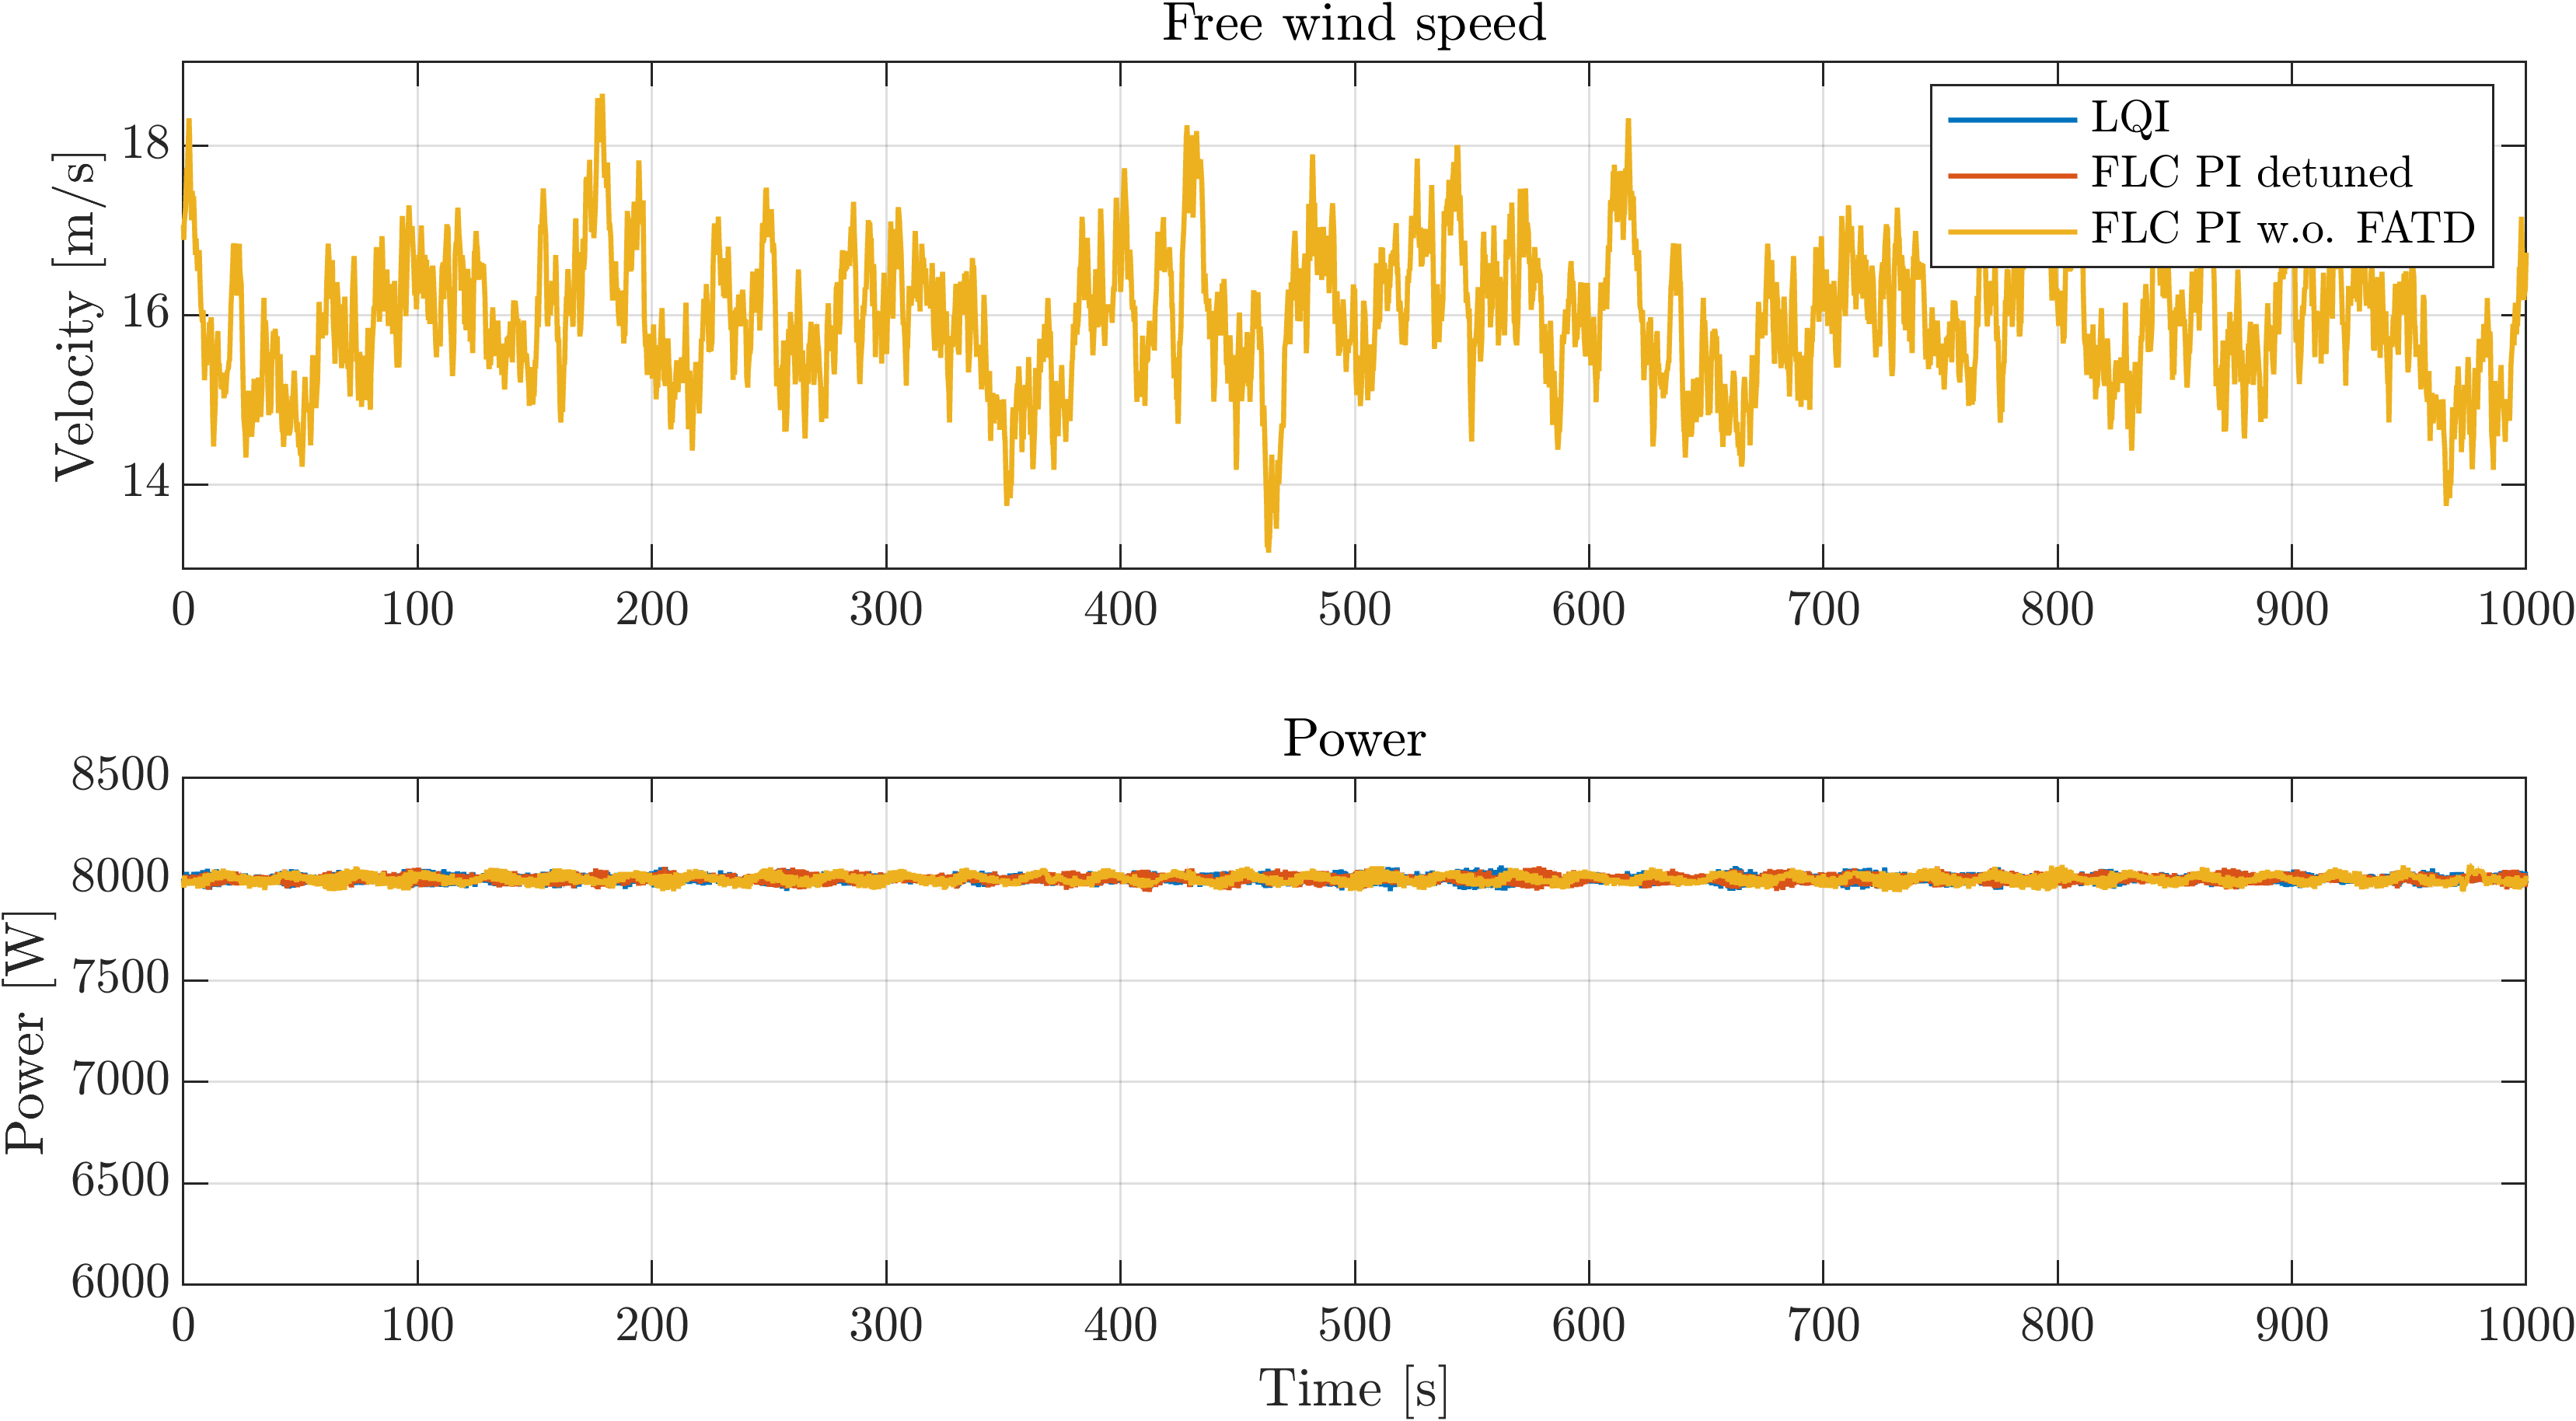
\includegraphics[width=0.7\linewidth]{Graphics/TestResults/VTSplotting/1_wind_pow.png}
	\caption{VTS simulation results showing the free wind speed and the power output of all three controllers. The mean wind speed is 16 m/s and the power output is constant around the nominal 8 MW}
	\label{fig:vts_1_wind_pow}
\end{figure}
\cref{fig:vts_2_fftazi} shows a Fourier transform of the rotor azimuth which gives a clear picture of the 1P and 3P frequency locations.
\begin{figure}[ht]
	\centering
	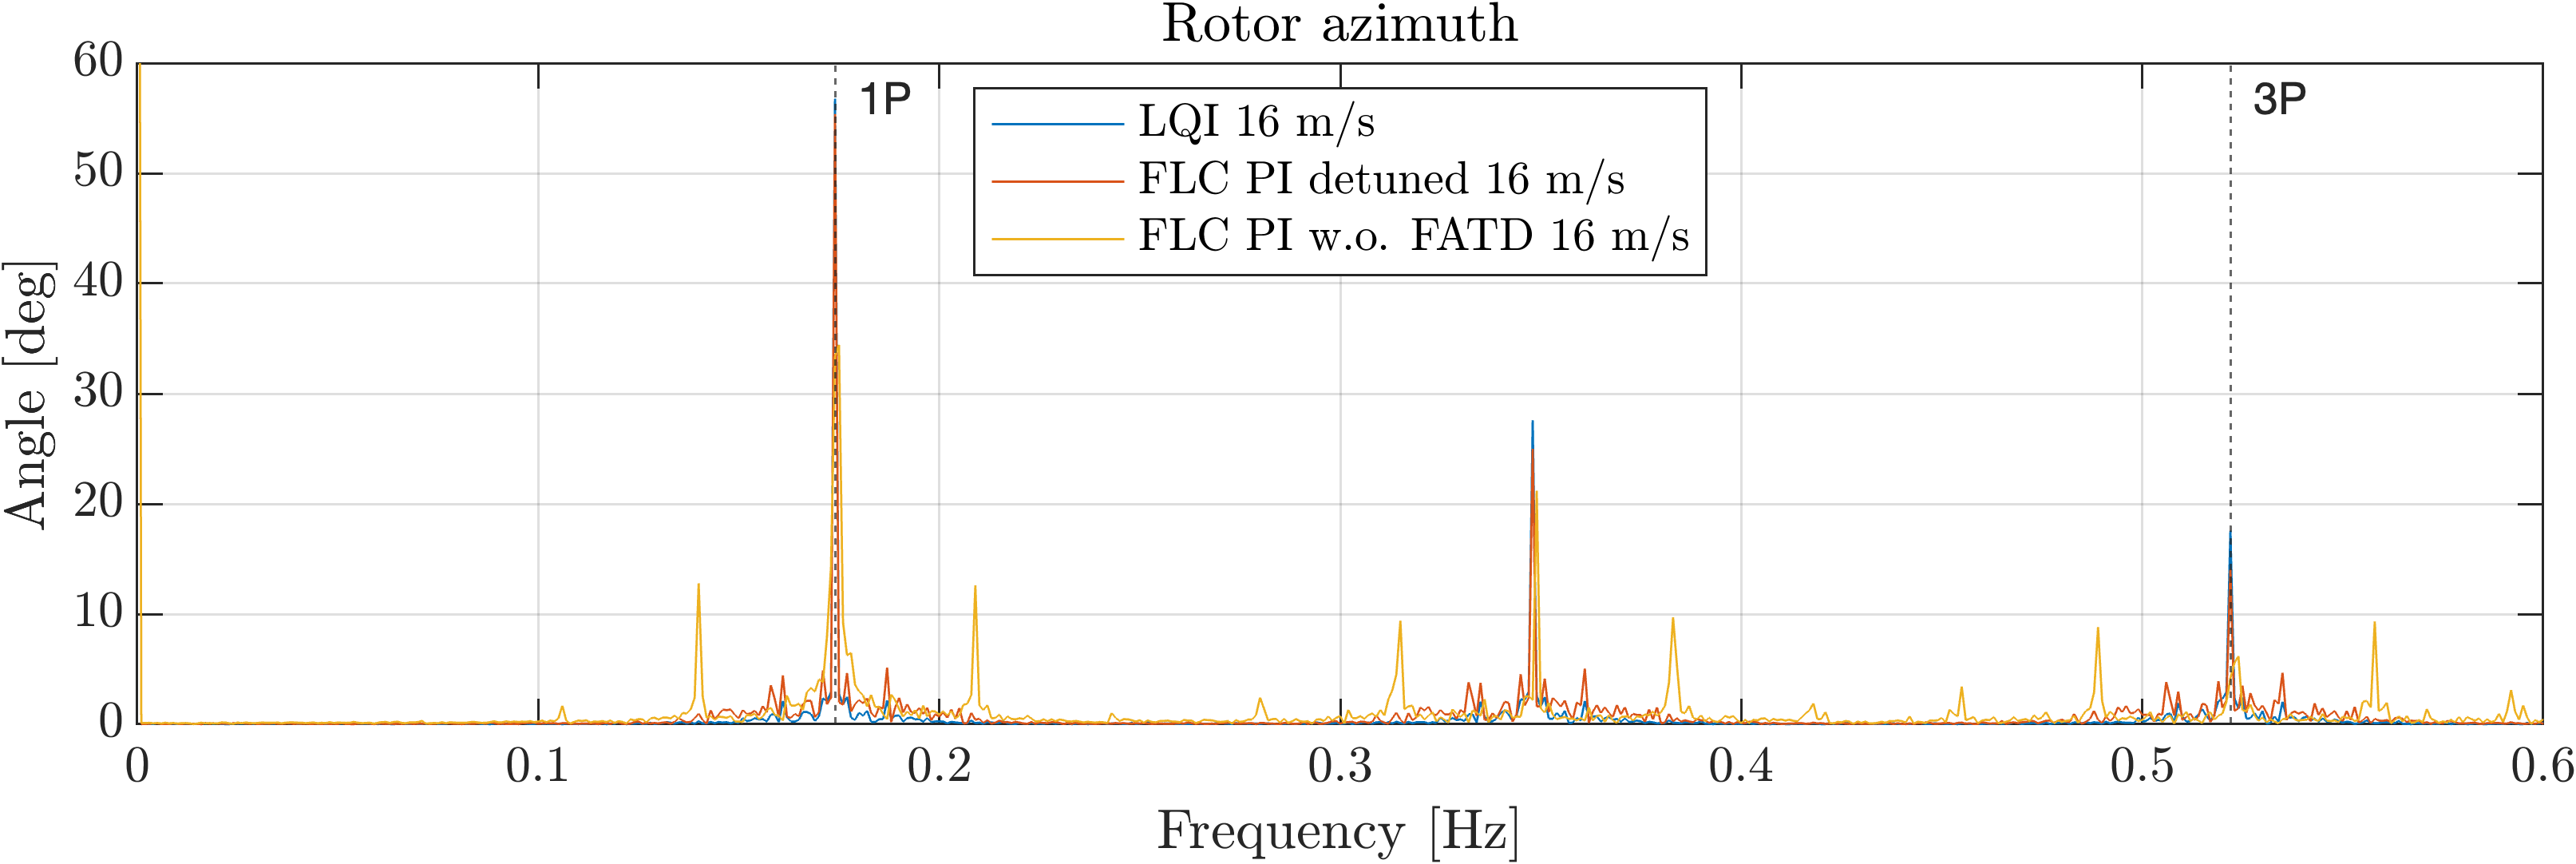
\includegraphics[width=0.7\linewidth]{Graphics/TestResults/VTSplotting/2_fftazi.png}
	\caption{VTS simulation results showing the Fourier transform of the rotor azimuth which clearly shows the 1P, 2P and 3P frequencies.}
	\label{fig:vts_2_fftazi}
\end{figure}

\cref{fig:vts_3_th_w_py_vy} contains four subplots: The pitch angle of blade 1, the generator speed, the fore-aft tower top position and the fore-aft tower top velocity. The blade pitch is included to evaluate blade pitch actuation and a lower blade pitch activity is ideal since it results in less mechanical wear. The generator speed set-point is set at 400 rpm and a lower absolute tracking error is better. The fore-aft (y-axis) tower top position and velocity should ideally be constant. It is readily visible that the fixed-bottom tuned FLC PI controller without FATD performs extremely poorly as it amplifies the fore-aft motion extensively. The oscillations are present in the whole system and an obvious conclusion is that it is infeasible to use the fixed-bottom tuned FLC controller in a real WT. The detuned FLC controller and the LQI controller perform much better with greatly reduced fore-aft motion. When observing the fft of the fore-aft velocity in \cref{fig:vts_4_fft_py} the eigenfrequency of the floater is readily visible at around 0.035 Hz.

\begin{figure}[h]
	\centering
	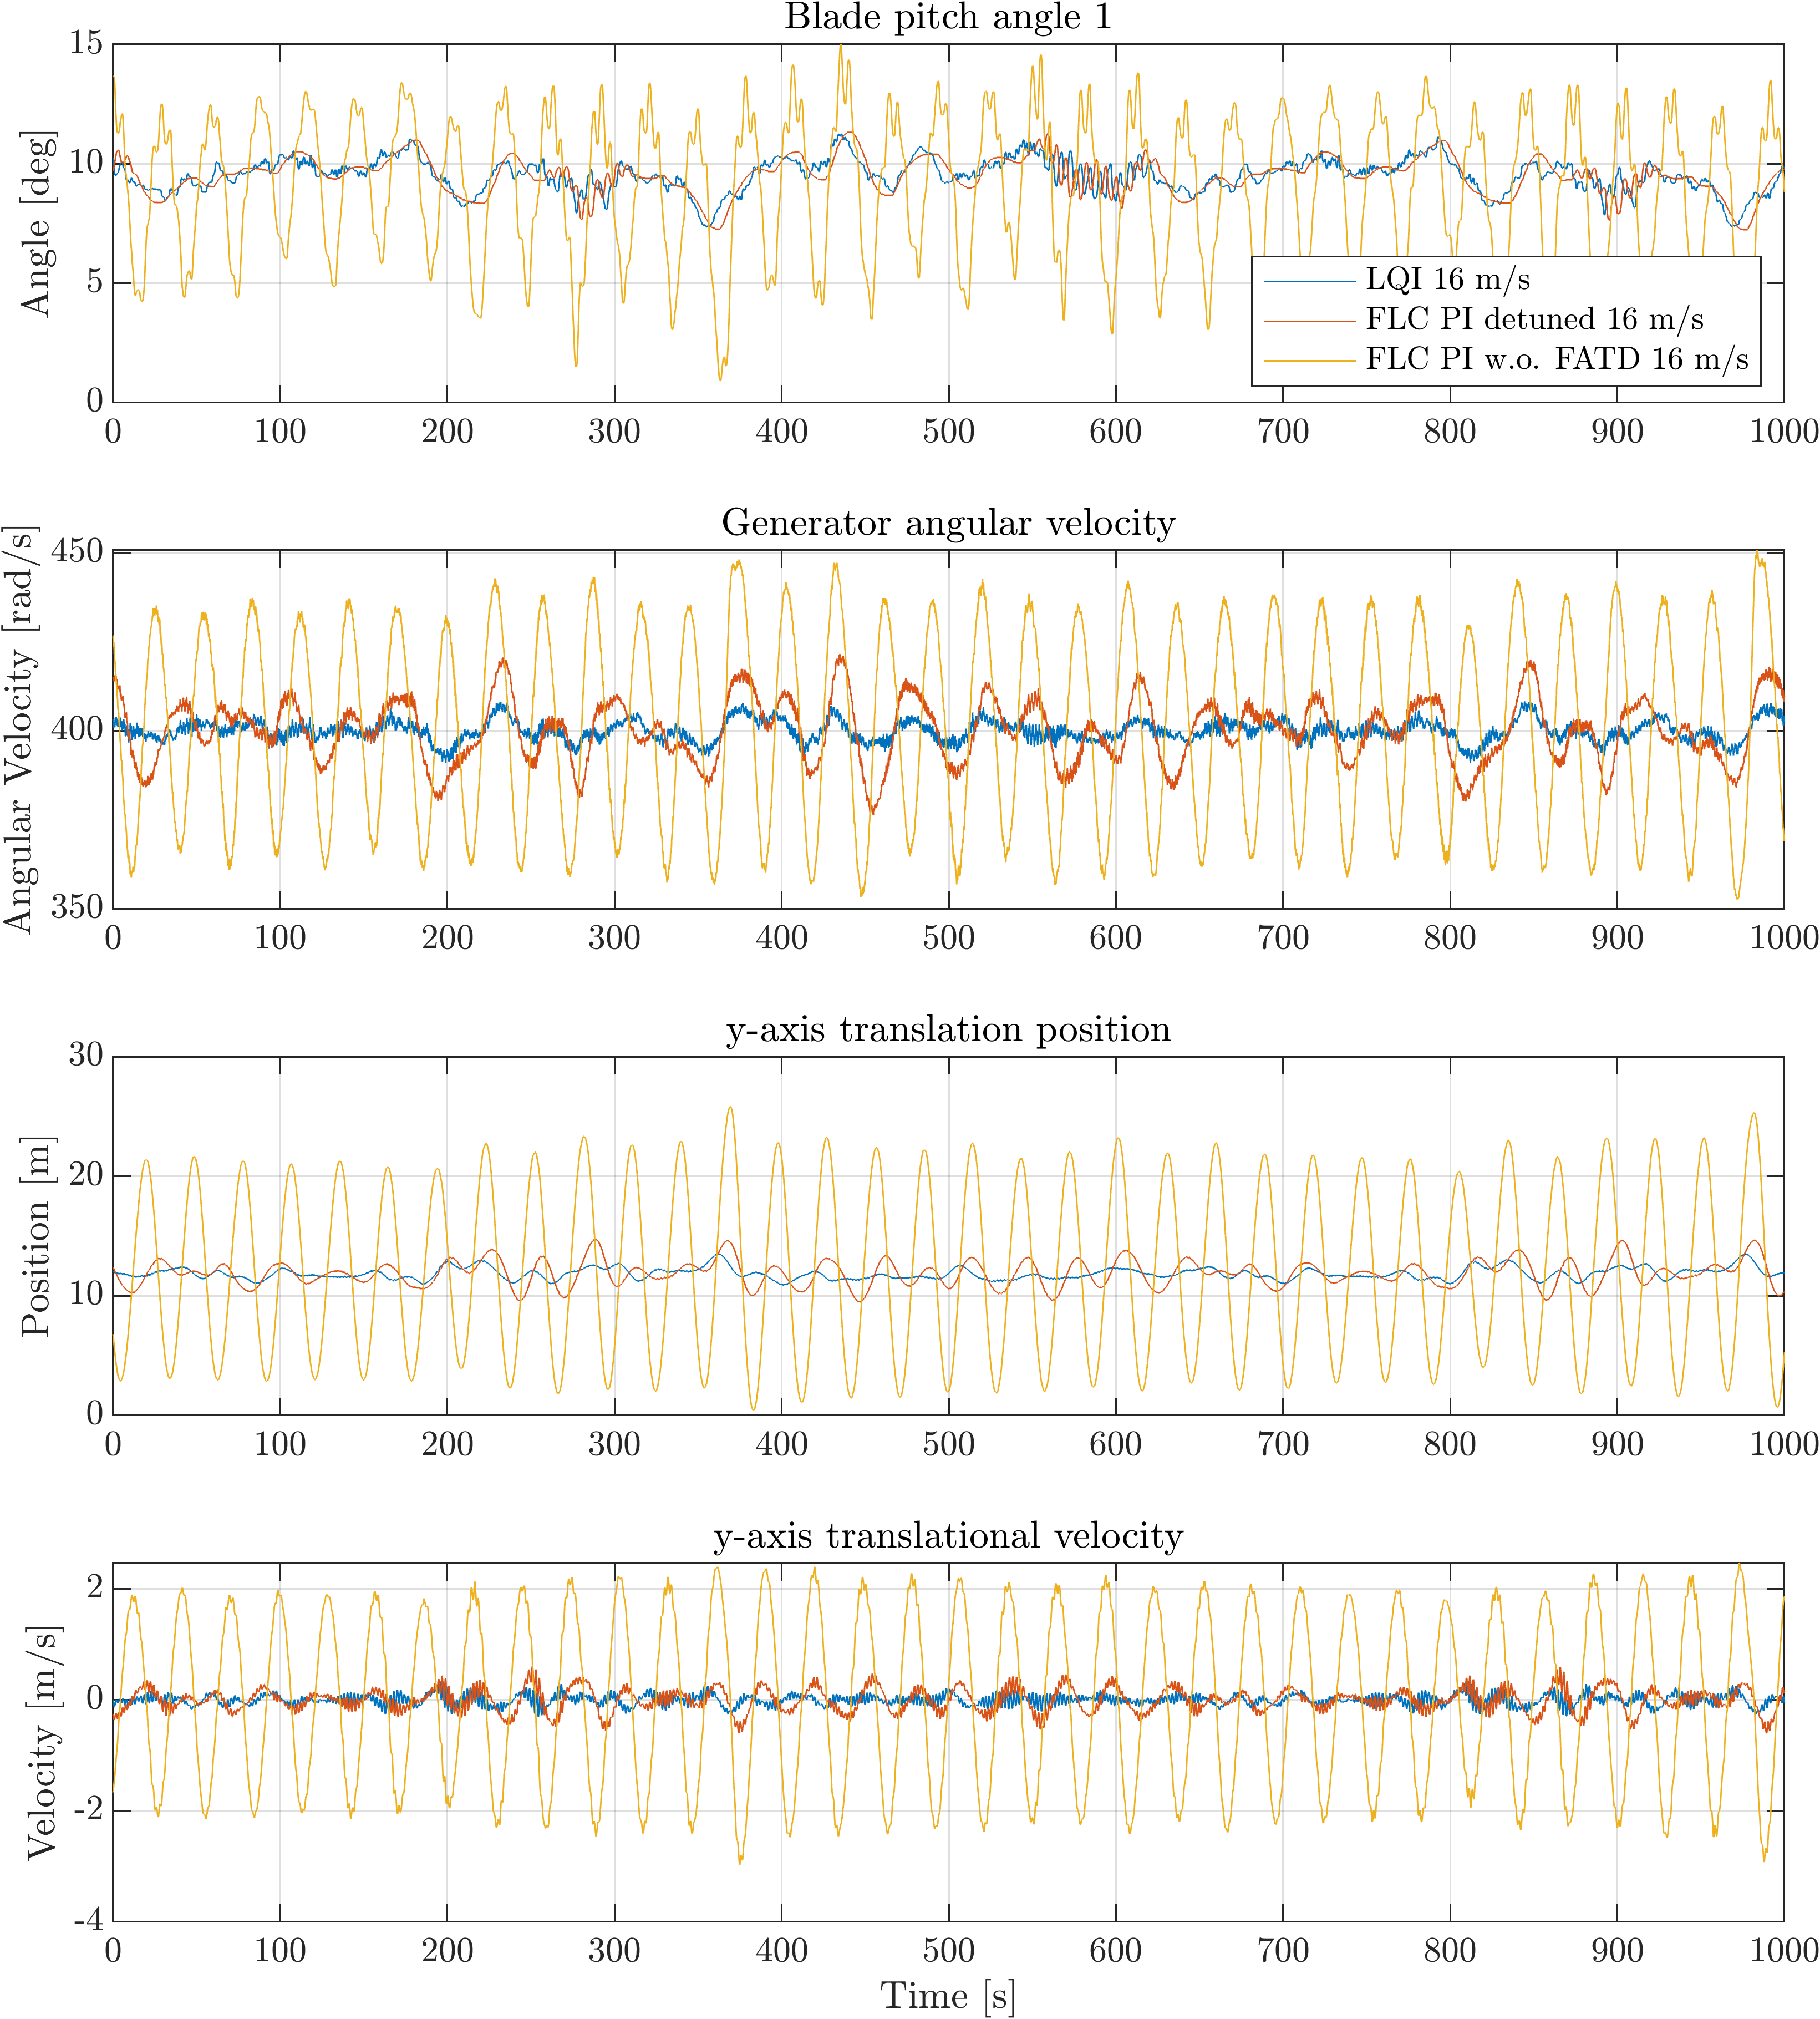
\includegraphics[width=0.7\linewidth]{Graphics/TestResults/VTSplotting/3_th_w_py_vy.png}
	\caption{VTS simulation results of the blade pitch, generator speed, fore-aft position and velocity. The fixed-bottom tuned FLC controller without FATD (yellow trace) is oscillating extensively in comparison to the LQI and detuned FLC controller.}
	\label{fig:vts_3_th_w_py_vy}
\end{figure}
\begin{figure}[h]
	\centering
	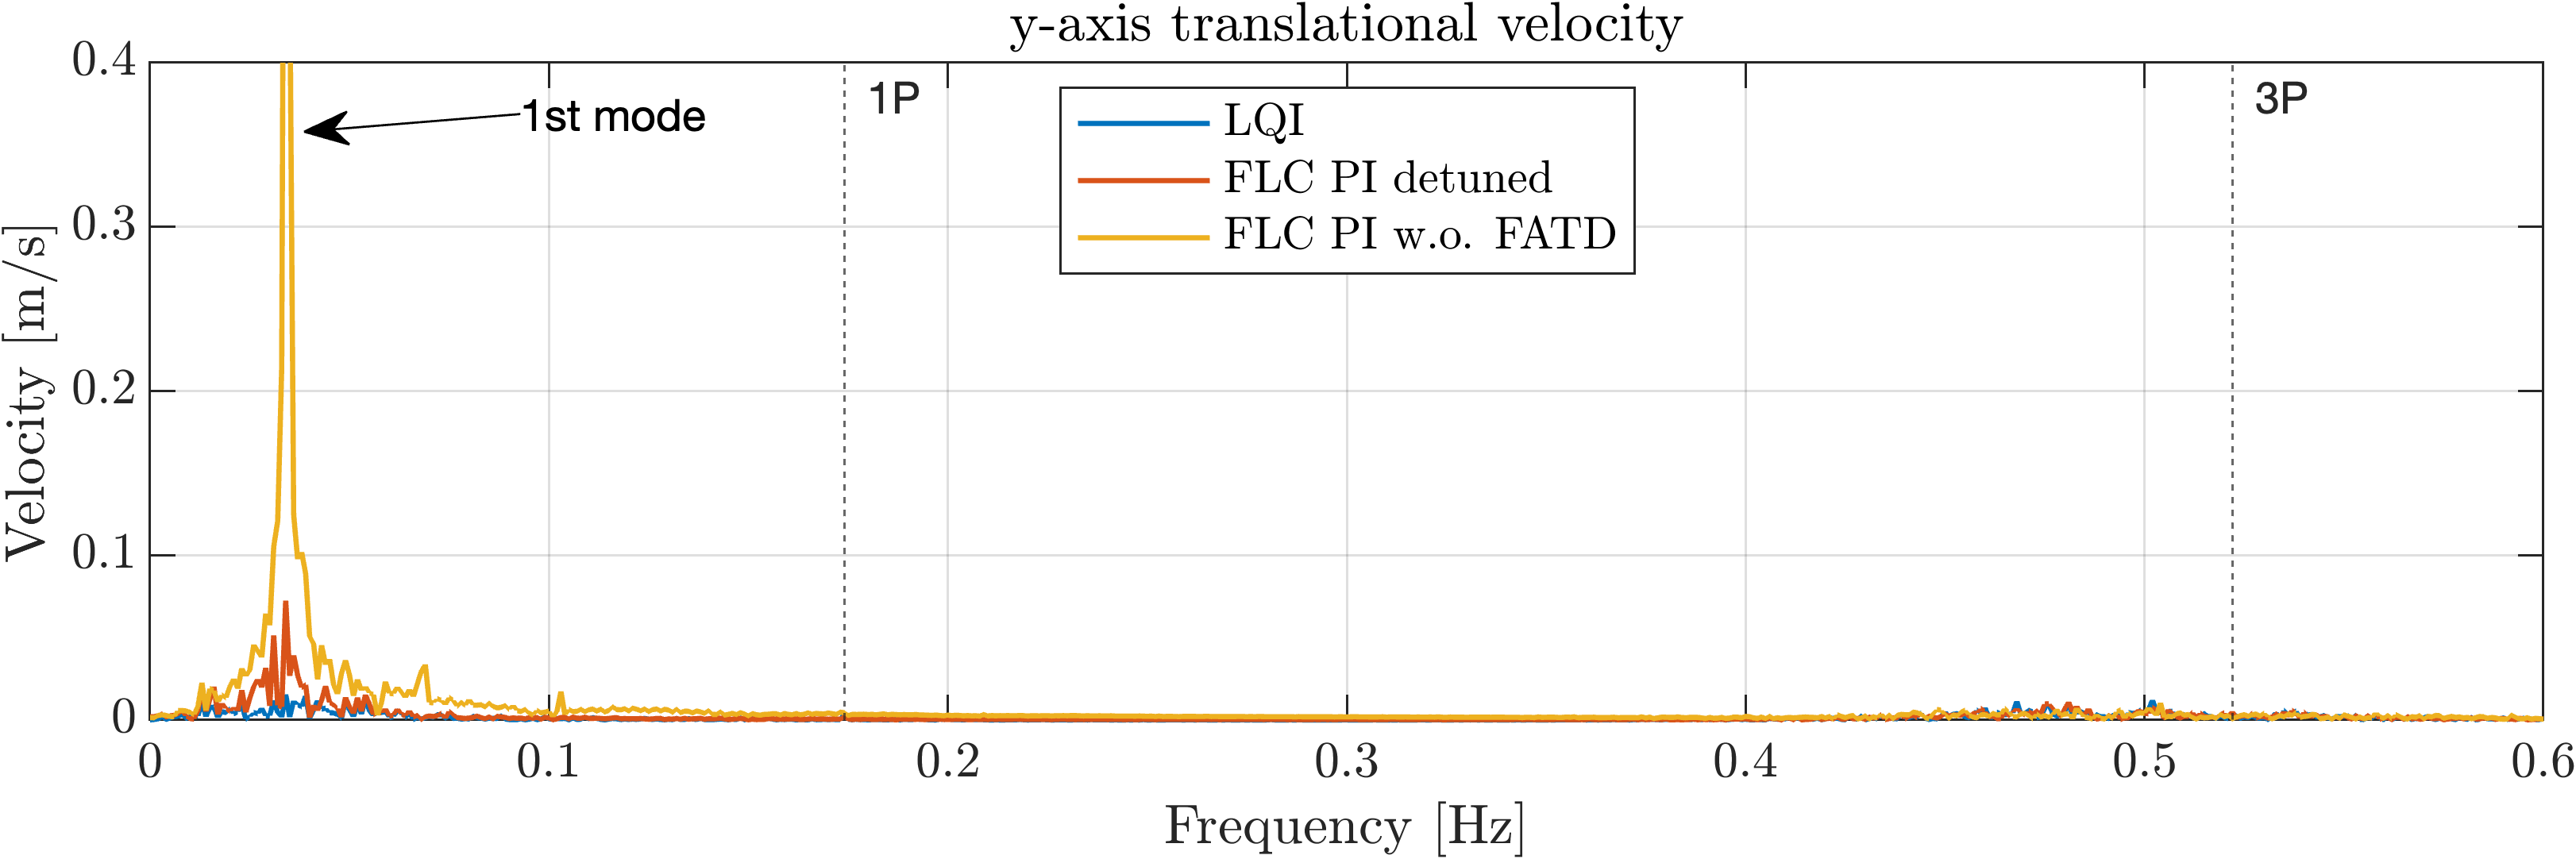
\includegraphics[width=0.7\linewidth]{Graphics/TestResults/VTSplotting/4_fft_py.png}
	\caption{VTS simulation results with the Fourier transform of the fore-aft velocity. The eigenfrequency component is readily visible on especially the fixed-bottom tuned FLC controller (yellow trace).}
	\label{fig:vts_4_fft_py}
\end{figure}

Due to the large oscillations of the fixed-bottom FLC PI controller it is difficult to compare the performance of the LQI controller with the detuned FLC PI controller. In \cref{fig:vts_10_th_w_py_vy} the fixed-bottom FLC controller trace is left out for easier comparison of the two remaining controllers. From this figure it can be observed that the LQI controller tracks the generator set-point the best due to the smaller absolute size of the tracking error. The fore-aft position oscillations are also dampened much better. The blade pitch angle actuation is largely the same with regards to the greater slow oscillations but smaller higher frequency oscillations seem to be present in the LQI controller. When observing the fore-aft velocity relatively fast oscillations seem to be present with both controllers. This behaviour is examined later. When observing the Fourier transform in \cref{fig:vts_11_fft_th_w_py_vy} zoomed in around the eigenfrequency it is apparent that the LQI controller performs the best in dampening the fore-aft motion. A lower actuator activity is even observed in the majority of the frequencies around the eigenfrequency.
\begin{figure}[h]
	\centering
	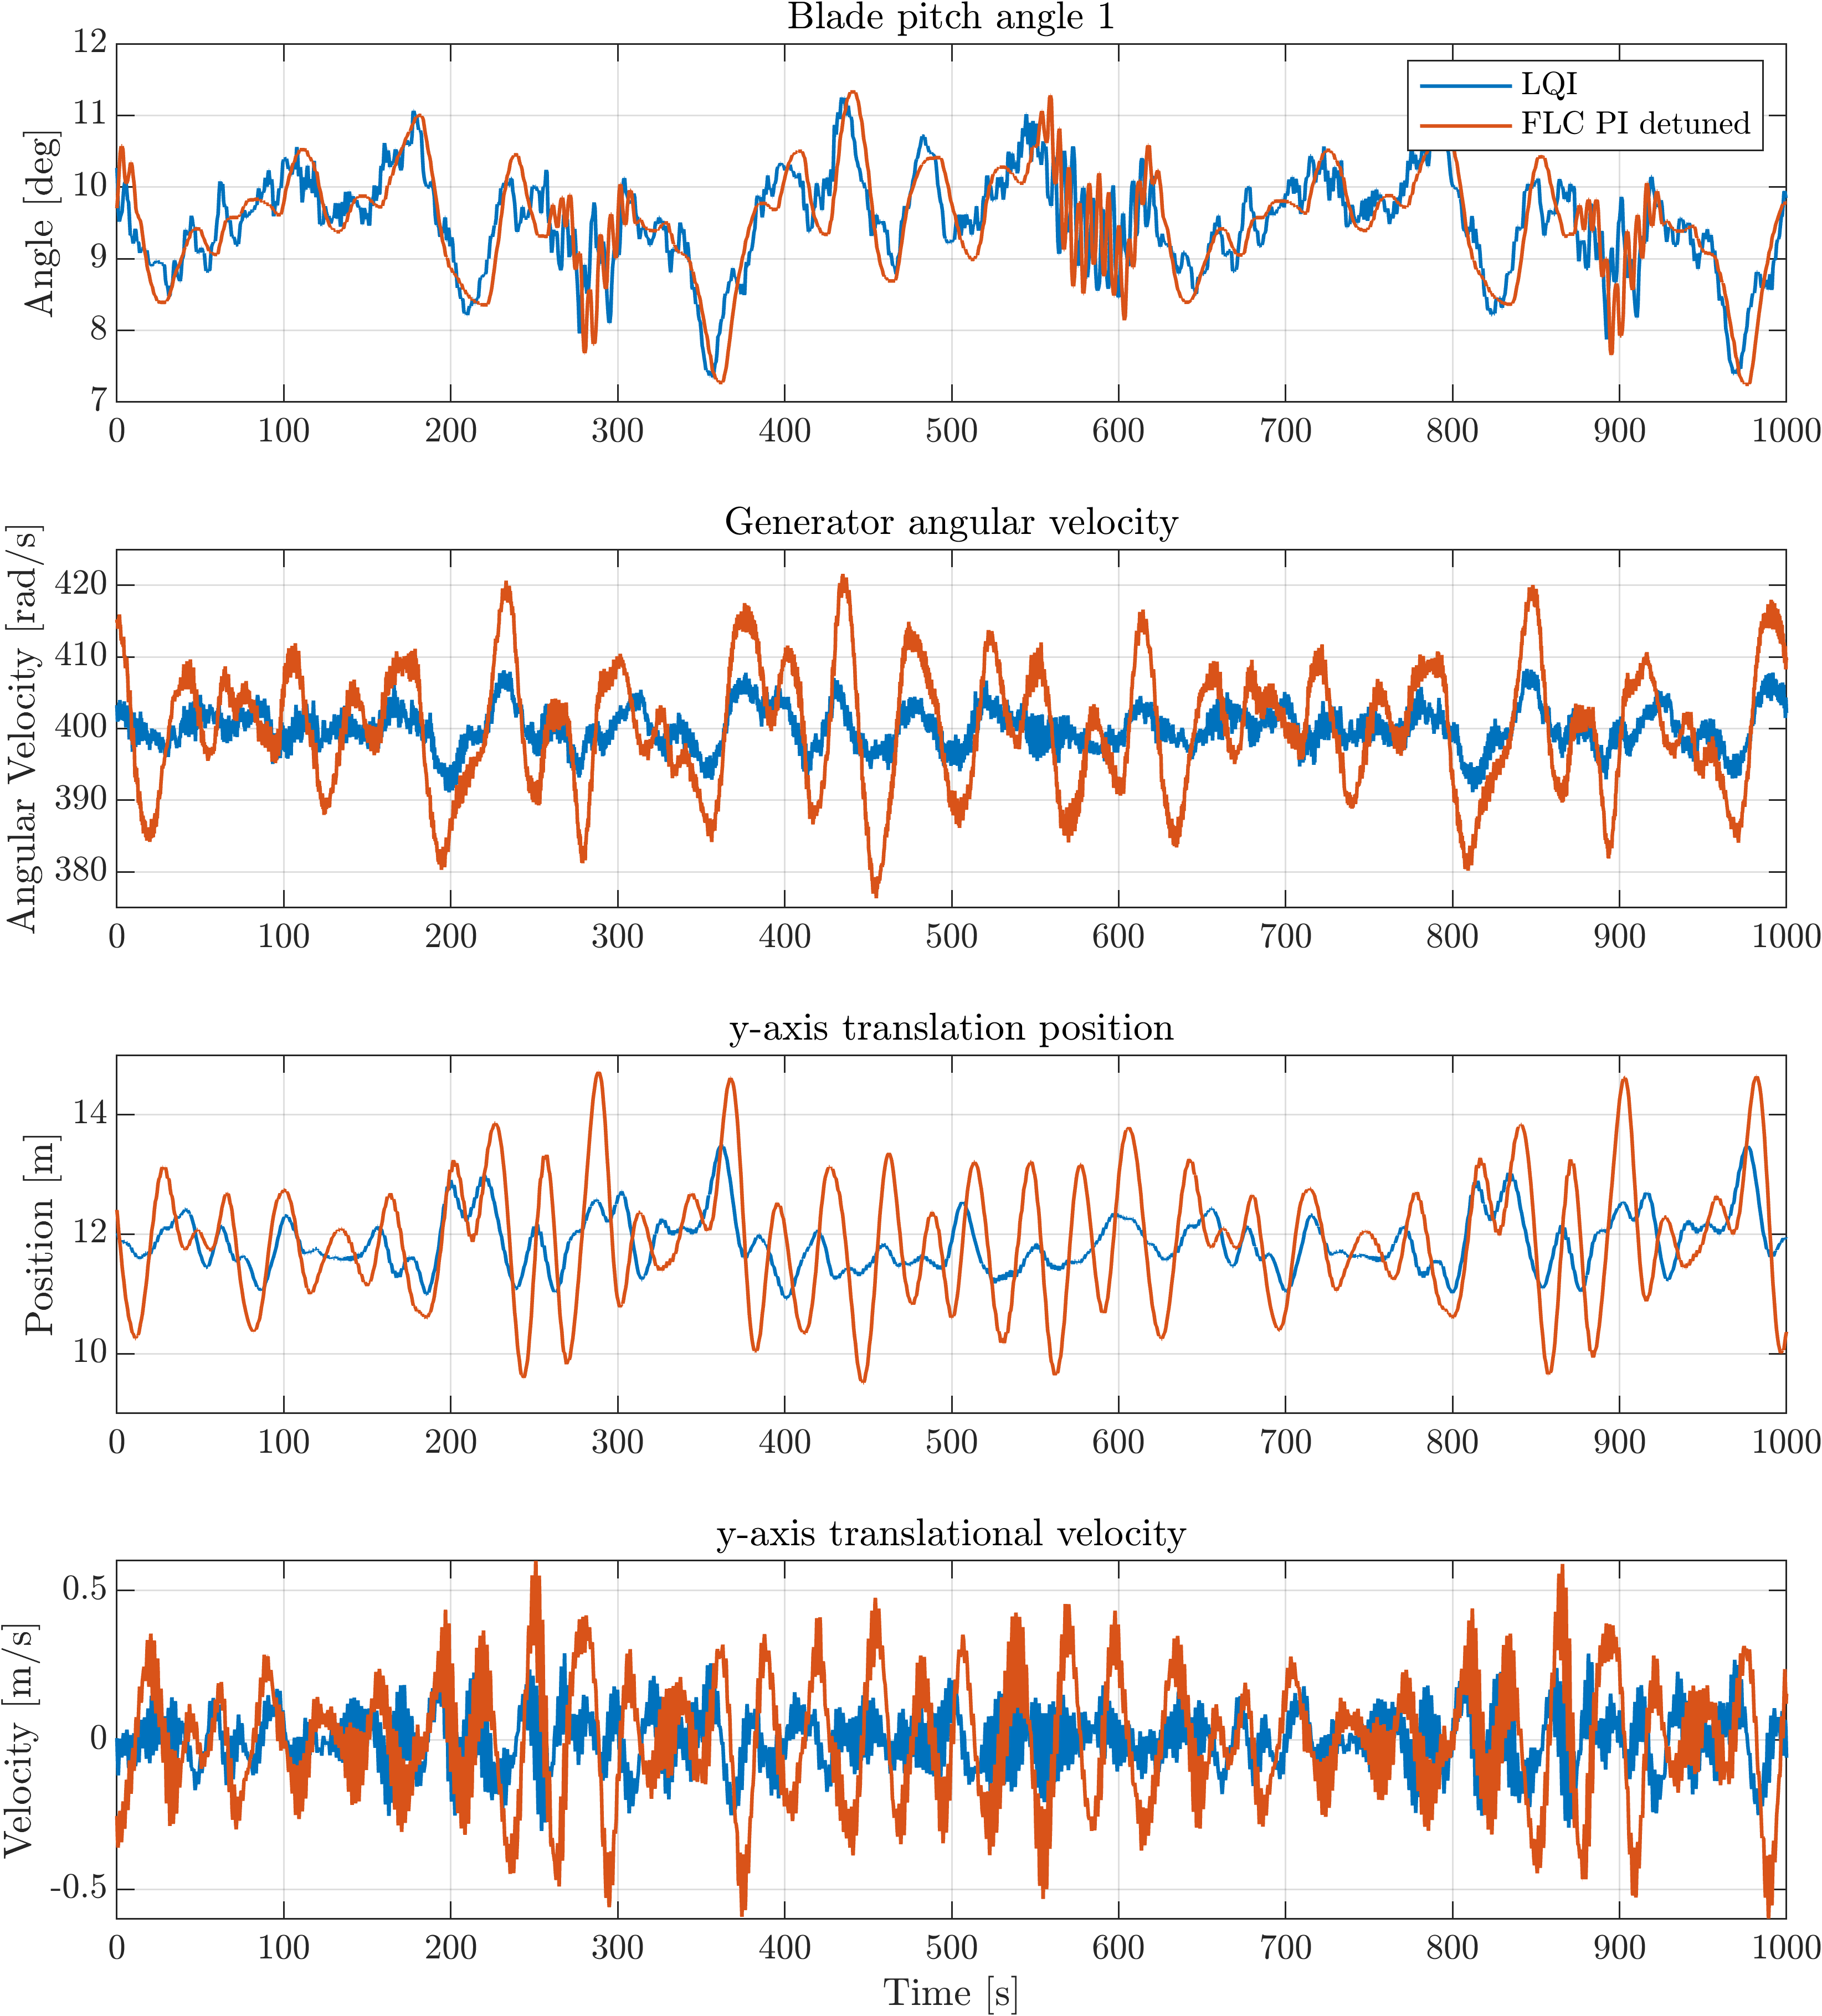
\includegraphics[width=0.7\linewidth]{Graphics/TestResults/VTSplotting/10_th_w_py_vy.png}
	\caption{VTS simulation results of the blade pitch, rotor speed, fore-aft position and velocity. Greater performance is achieved with the LQI controller in all aspects besides the higher frequency component on the blade pitch angle.}
	\label{fig:vts_10_th_w_py_vy}
\end{figure}

\clearpage

\begin{figure}[h]
	\centering
	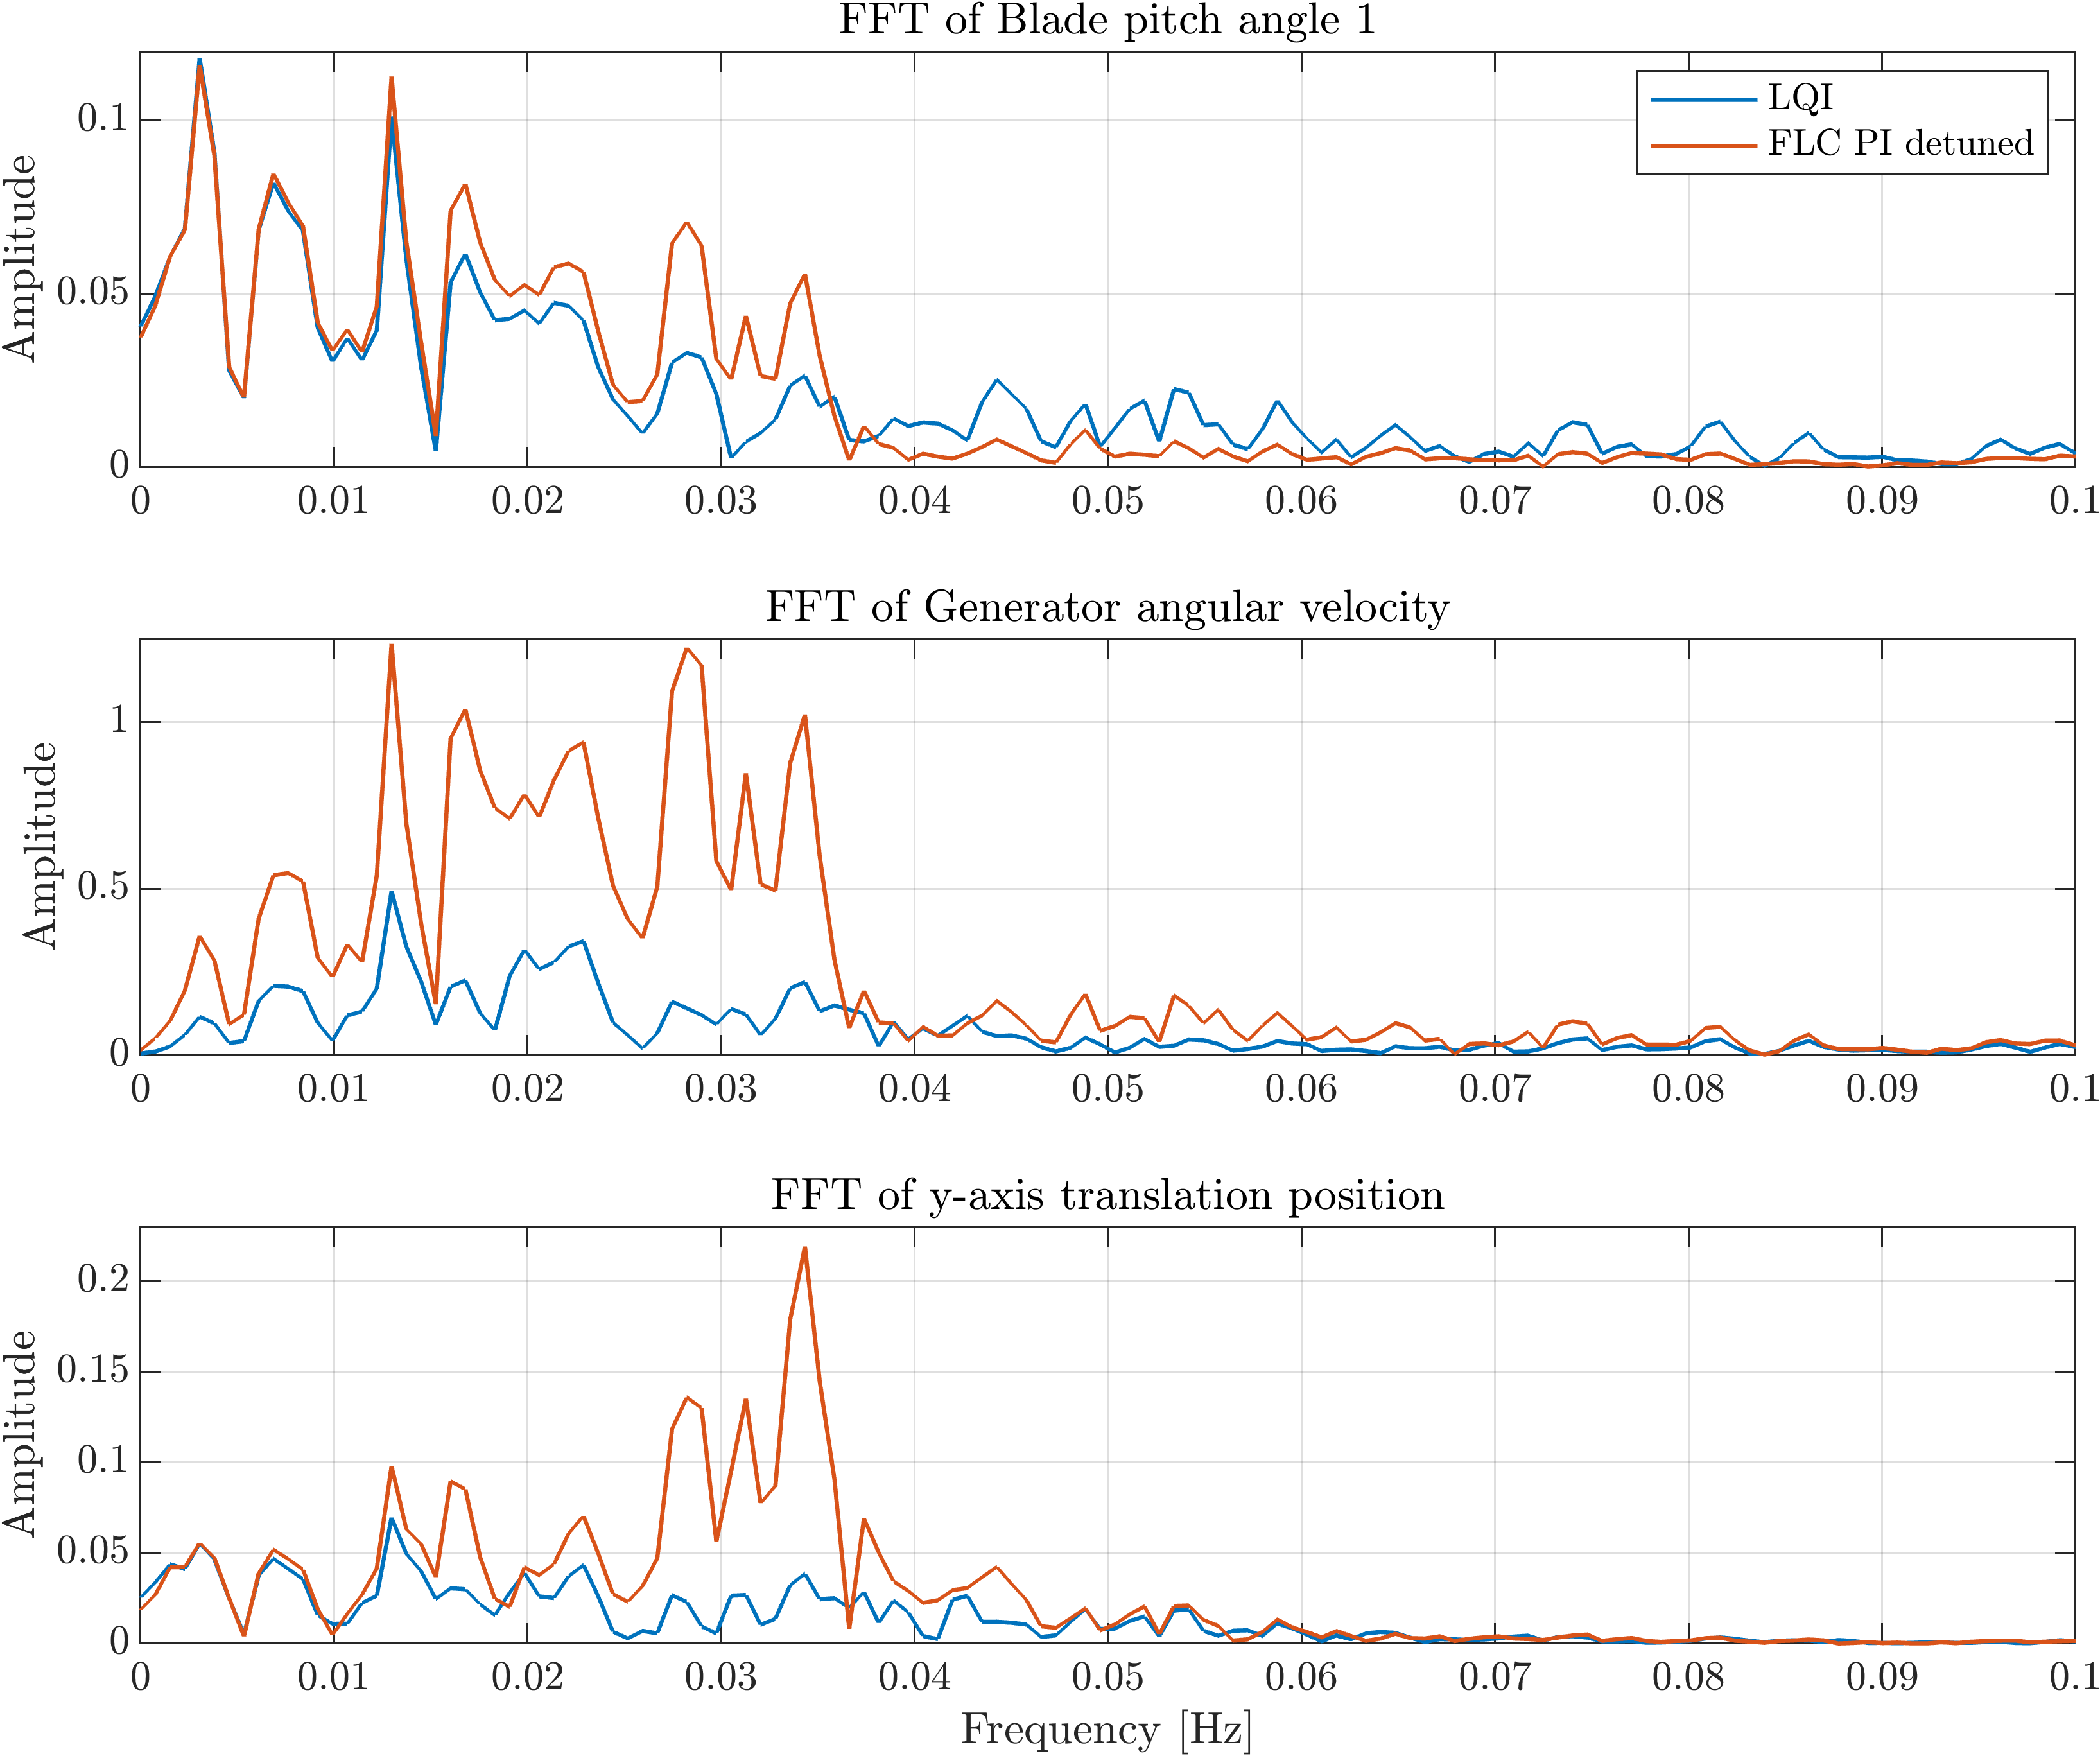
\includegraphics[width=0.7\linewidth]{Graphics/TestResults/VTSplotting/11_fft_th_w_py.png}
	\caption{VTS simulation results with the Fourier transform of the blade pitch, generator angular velocity and the fore-aft position. The fore-aft velocity is left out because the frequency content around the eigenfrequency is identical to the position.}
	\label{fig:vts_11_fft_th_w_py_vy}
\end{figure}

When looking at \cref{fig:vts_12_zoom_th_w_py_vy} the fore-aft velocity oscillations are obvious. They are present due to oscillations in the tower which is the second mode of a floating turbine as was illustrated earlier in \cref{fig:eigen_and_1p3p}. When observing the Fourier transform plot in \cref{fig:vts_13_zoom_fft_th_w_py_vy} which contains frequencies around 0.5 Hz these oscillations are seen around 0.45 to 0.49 Hz and are very close to the 3P frequencies around 0.5 to 0.55 Hz. The second mode's location close to the 3P frequency was also highlighted before in \cref{fig:vts_12_zoom_th_w_py_vy} and thus this does not come as a surprise. This large second mode oscillation is unwanted but also invisible to the LQI controller as it has not been modelled. Should it have been dampened the fore-aft model defined in \cref{sec:comp_foreaft_mod} should have included a second mass-spring-damper in series.
\begin{figure}[ht]
	\centering
	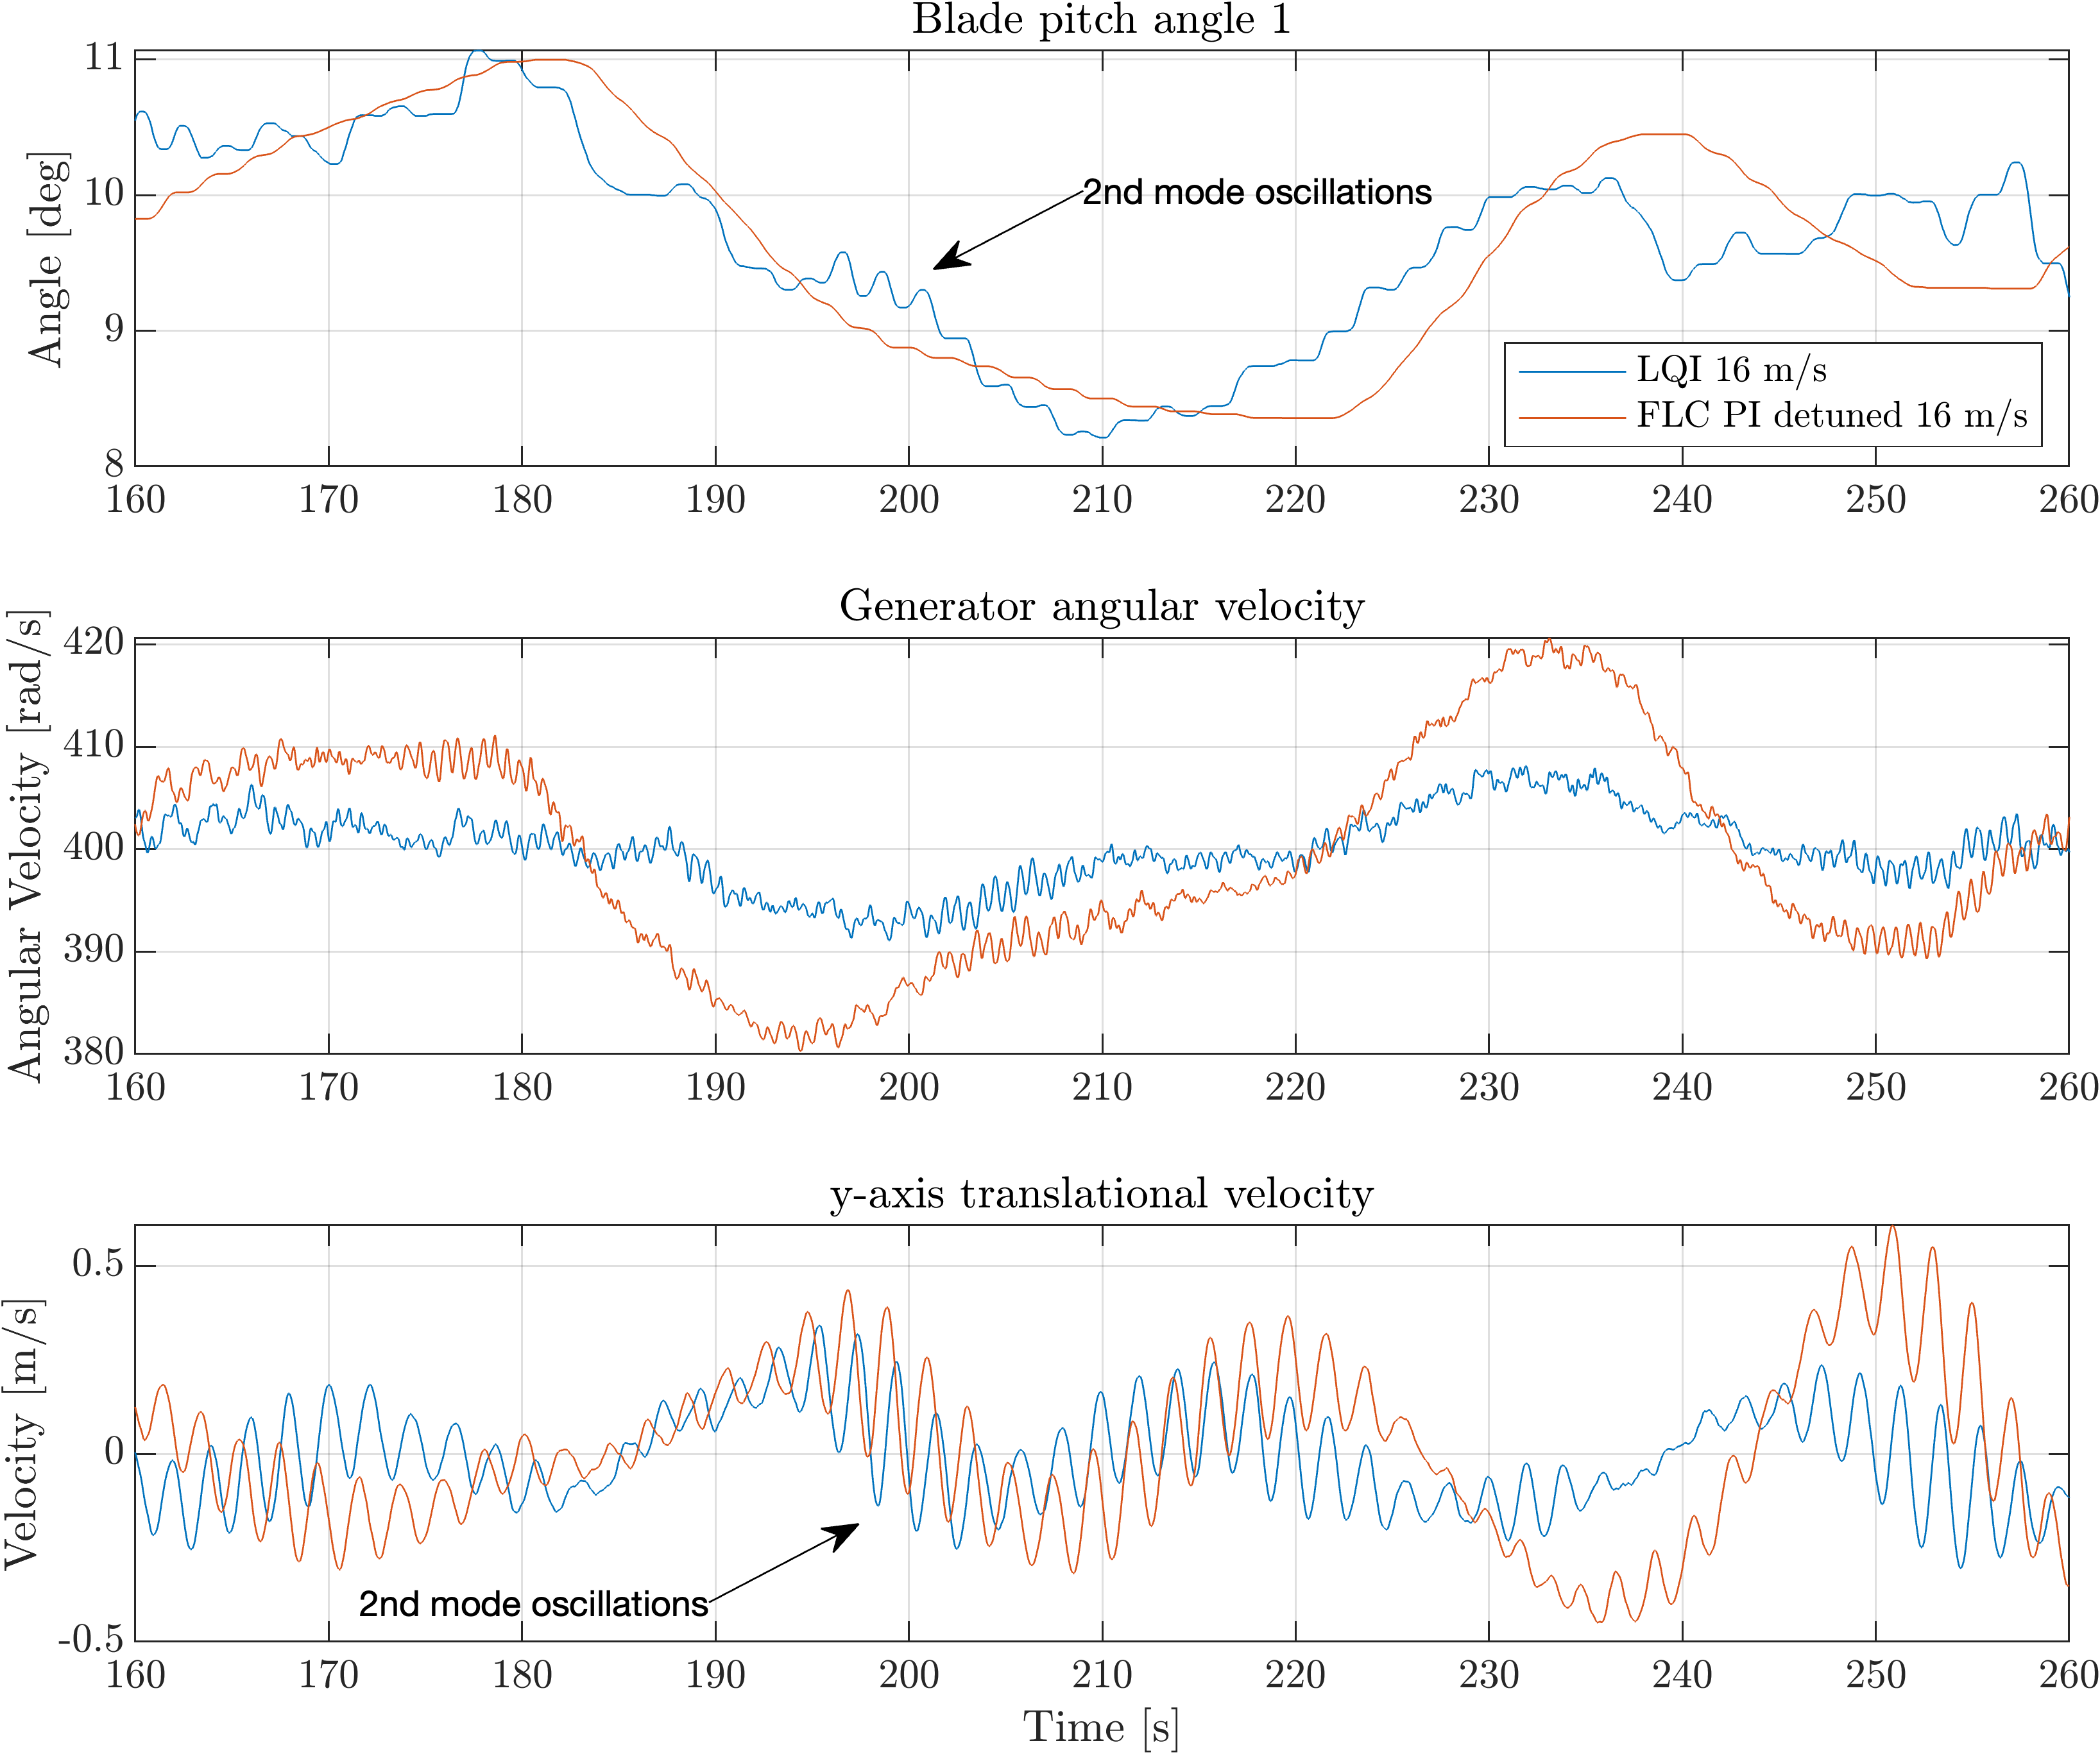
\includegraphics[width=0.7\linewidth]{Graphics/TestResults/VTSplotting/12_zoom_th_w_vy.png}
	\caption{VTS simulation results in a 100 second window at time 160 to 260 seconds. The 2nd mode oscillations are visible in the fore-aft velocity and due to the fore-aft velocity feedback they are transferred to the pitch angle.}
	\label{fig:vts_12_zoom_th_w_py_vy}
\end{figure}
\begin{figure}[ht]
	\centering
	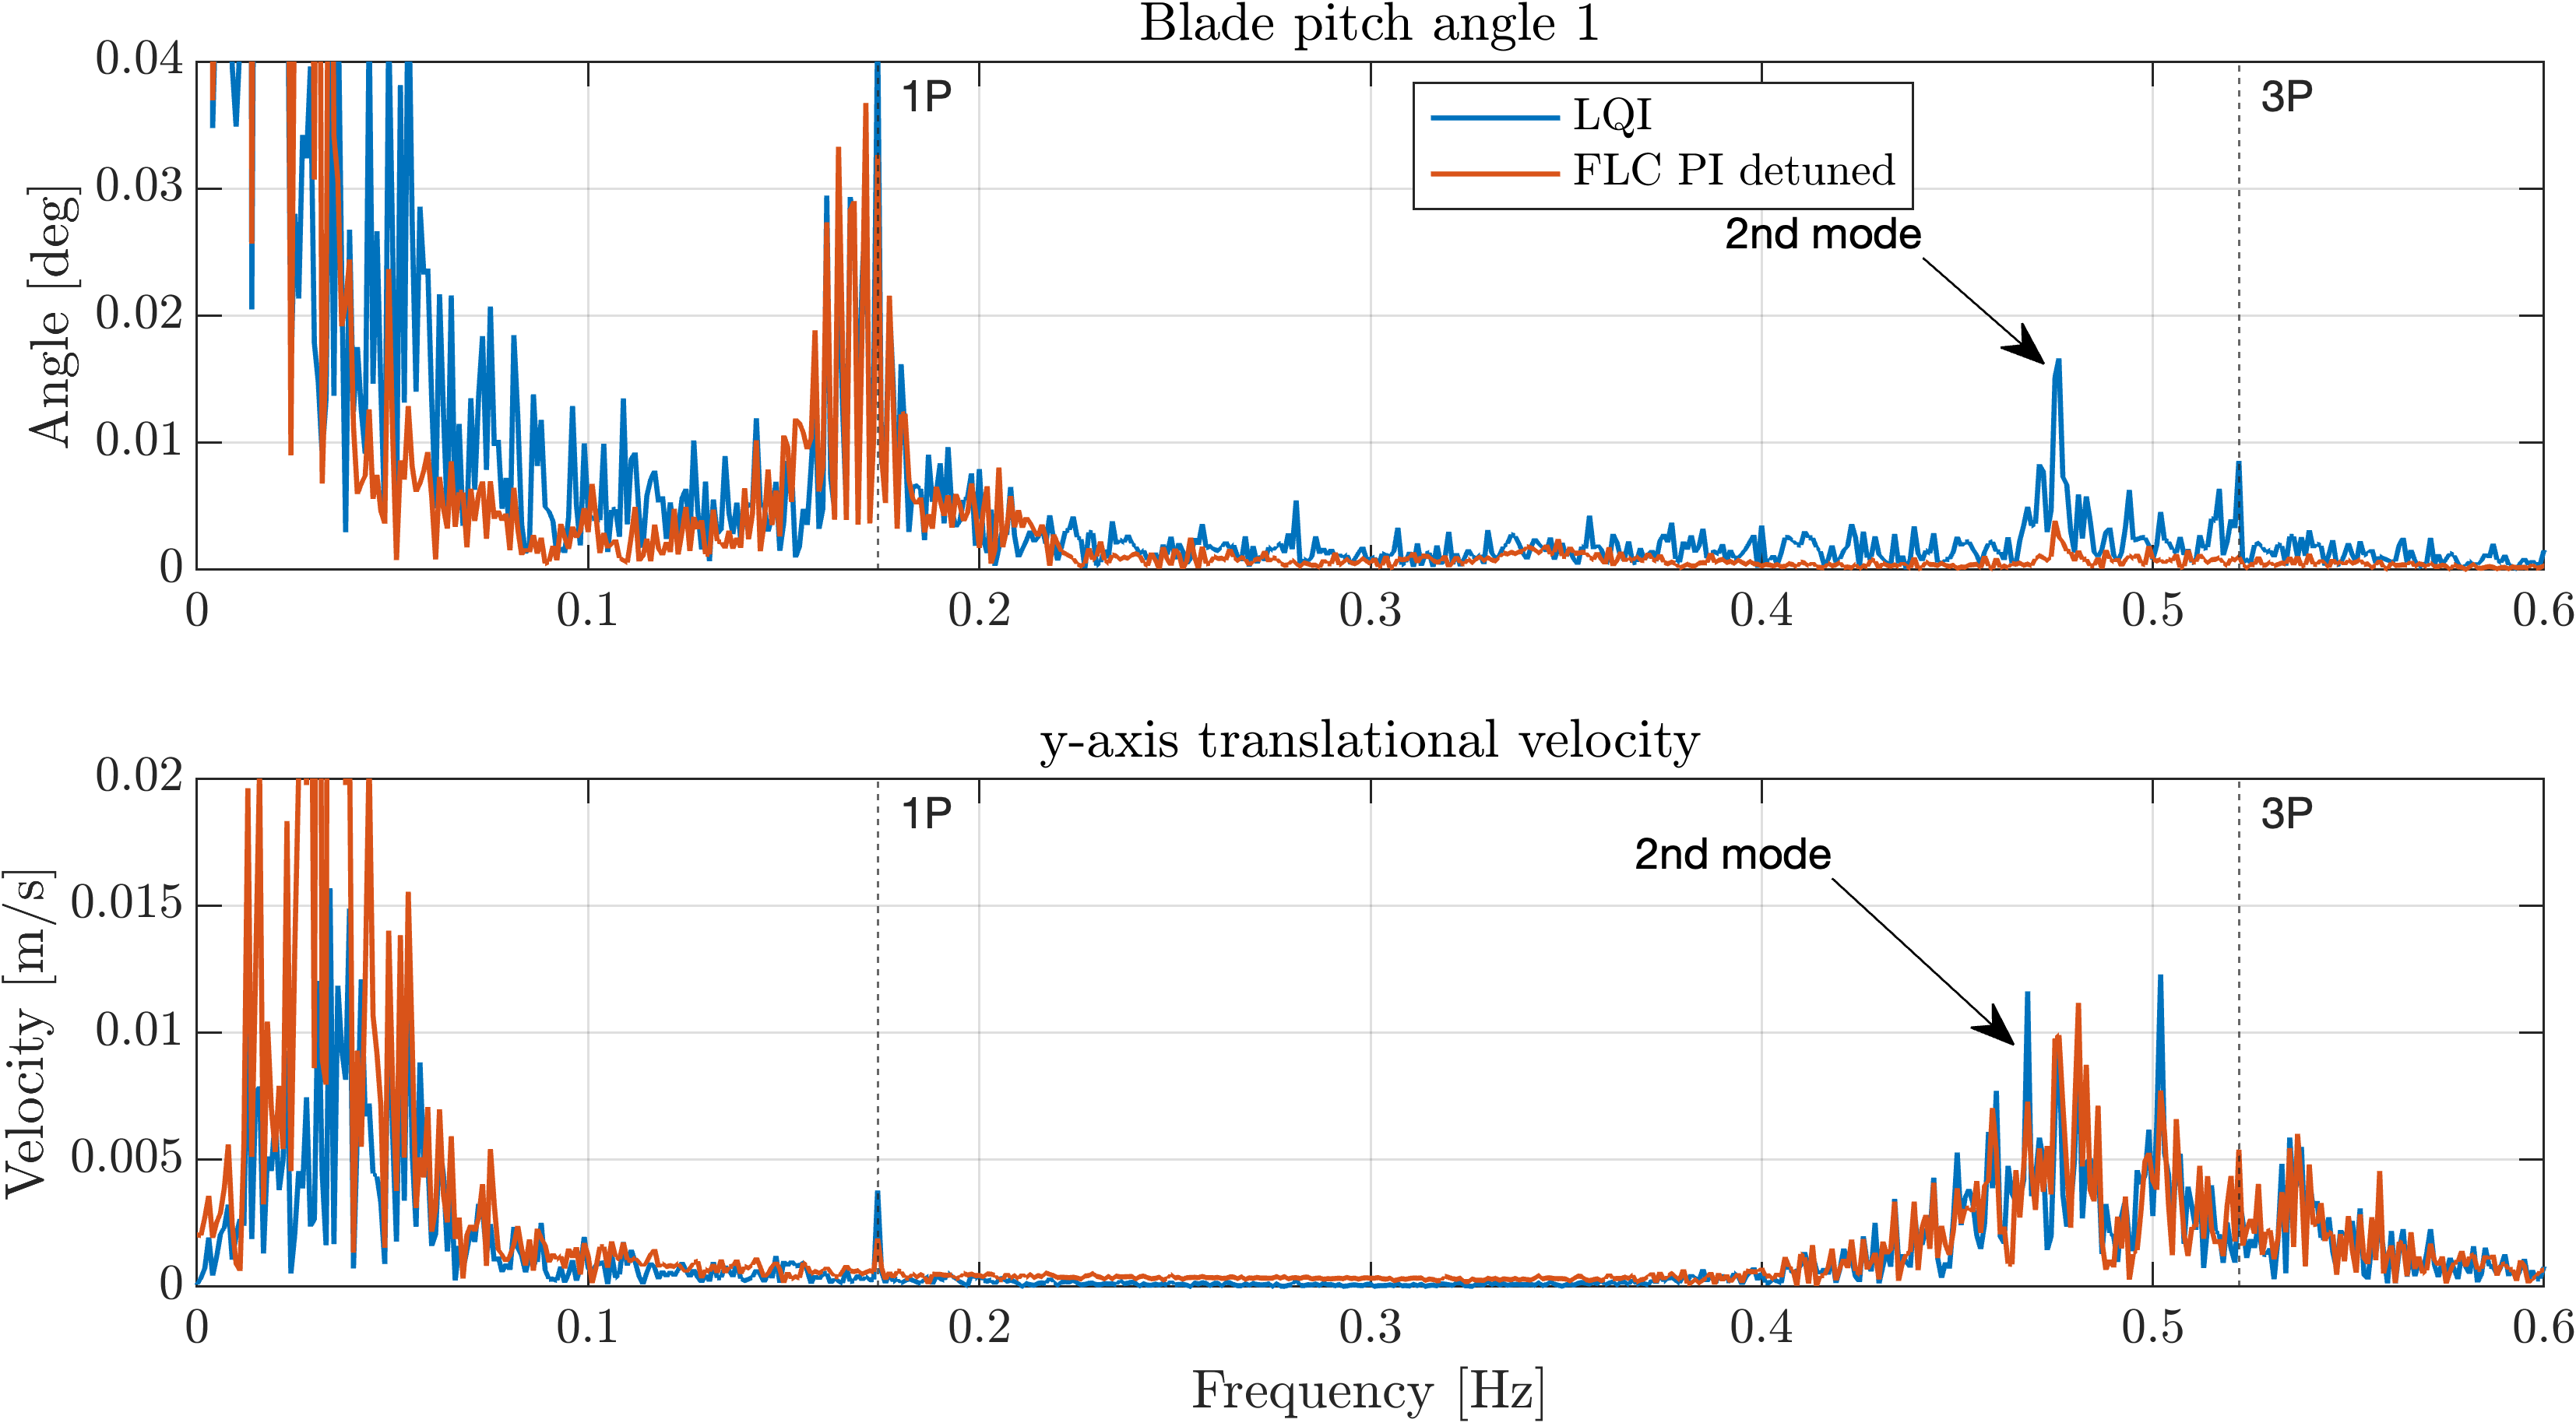
\includegraphics[width=0.7\linewidth]{Graphics/TestResults/VTSplotting/13_zoom_fft_th_vy.png}
	\caption{VTS simulation results with the Fourier transform which includes frequencies around 0.5 Hz. Second mode oscillations are obvious in the neighbourhood of 0.45 to 0.49 Hz on both simulations and they are translated into the blade pitch with the LQI controller.}
	\label{fig:vts_13_zoom_fft_th_w_py_vy}
\end{figure}

\clearpage
\subsection{Results: 12, 16 and 26 m/s LQI OP performance comparison}
It is of interest to see whether using a model for the controller at other OPs yield a better controller performance at the other respective OPs despite not further tuning the LQI weights. Only a single convenient OP has been considered in the project so far since gain scheduling has been deemed out of scope. But recalculating the LQI controller gains for a different OP using the Vestas wtLin tool is convenient and therefore some results of the controller performance at other OPs are included. The LQI $ Q $ and $ R $ weights are not tuned for the other OPs but are left at the values which yielded the best performance at 16 m/s.

As mentioned the new wind speeds are 12 m/s and 26 m/s. Due to the larger rotor thrust sensitivity around nominal wind speed which can be observed in \cref{fig:thrust_vs_windspeed} greater instability is expected for the 12 m/s simulations. The WT controller will furthermore change between PLC and FLC as the wind speed observed by the rotor goes above and below the nominal wind speed. This is expected to decrease stability and worsen overall performance. At higher wind the rotor thrust sensitivity decreases and thus greater general stability and better performance is expected at 26 m/s.

In \cref{fig:vts_20_pow_th_w_py_vy} the 16, 12 and 26 m/s OP LQI controller parameter configurations are compared at a 12 m/s mean wind speed. As expected the power deviates from 8 MW due to the switching between PLC and FLC. The power fluctuations are largely the same except around 0 to 60 seconds and 610 to 670 seconds where the 12 m/s LQI configuration has some fluctuations not observed in the other two. When observing the fore-aft velocity in the bottom plot a slightly greater backwards velocity is present which would cause a lower observed wind speed at the rotor resulting in a dip into PLC. The blade pitch activity seems to be largely the same across the controllers. The rotor speed errors is better for the 12 m/s LQI controller in several places especially visible around 50 to 130 seconds and 650 to 730 seconds. The greater rotor speed tracking seems to come at the cost of slightly worse fore-aft motion dampening observed in the fore-aft position and velocity plots. Although when consulting the Fourier transform plot in \cref{fig:vts_21_fft_th_w_py_vy} the 12 m/s configuration seems to dampen almost all oscillations around the natural frequency better. Only 0 to 0.1 Hz is plotted since the frequency content for greater frequencies is mainly flat.

\begin{figure}[ht]
	\centering
	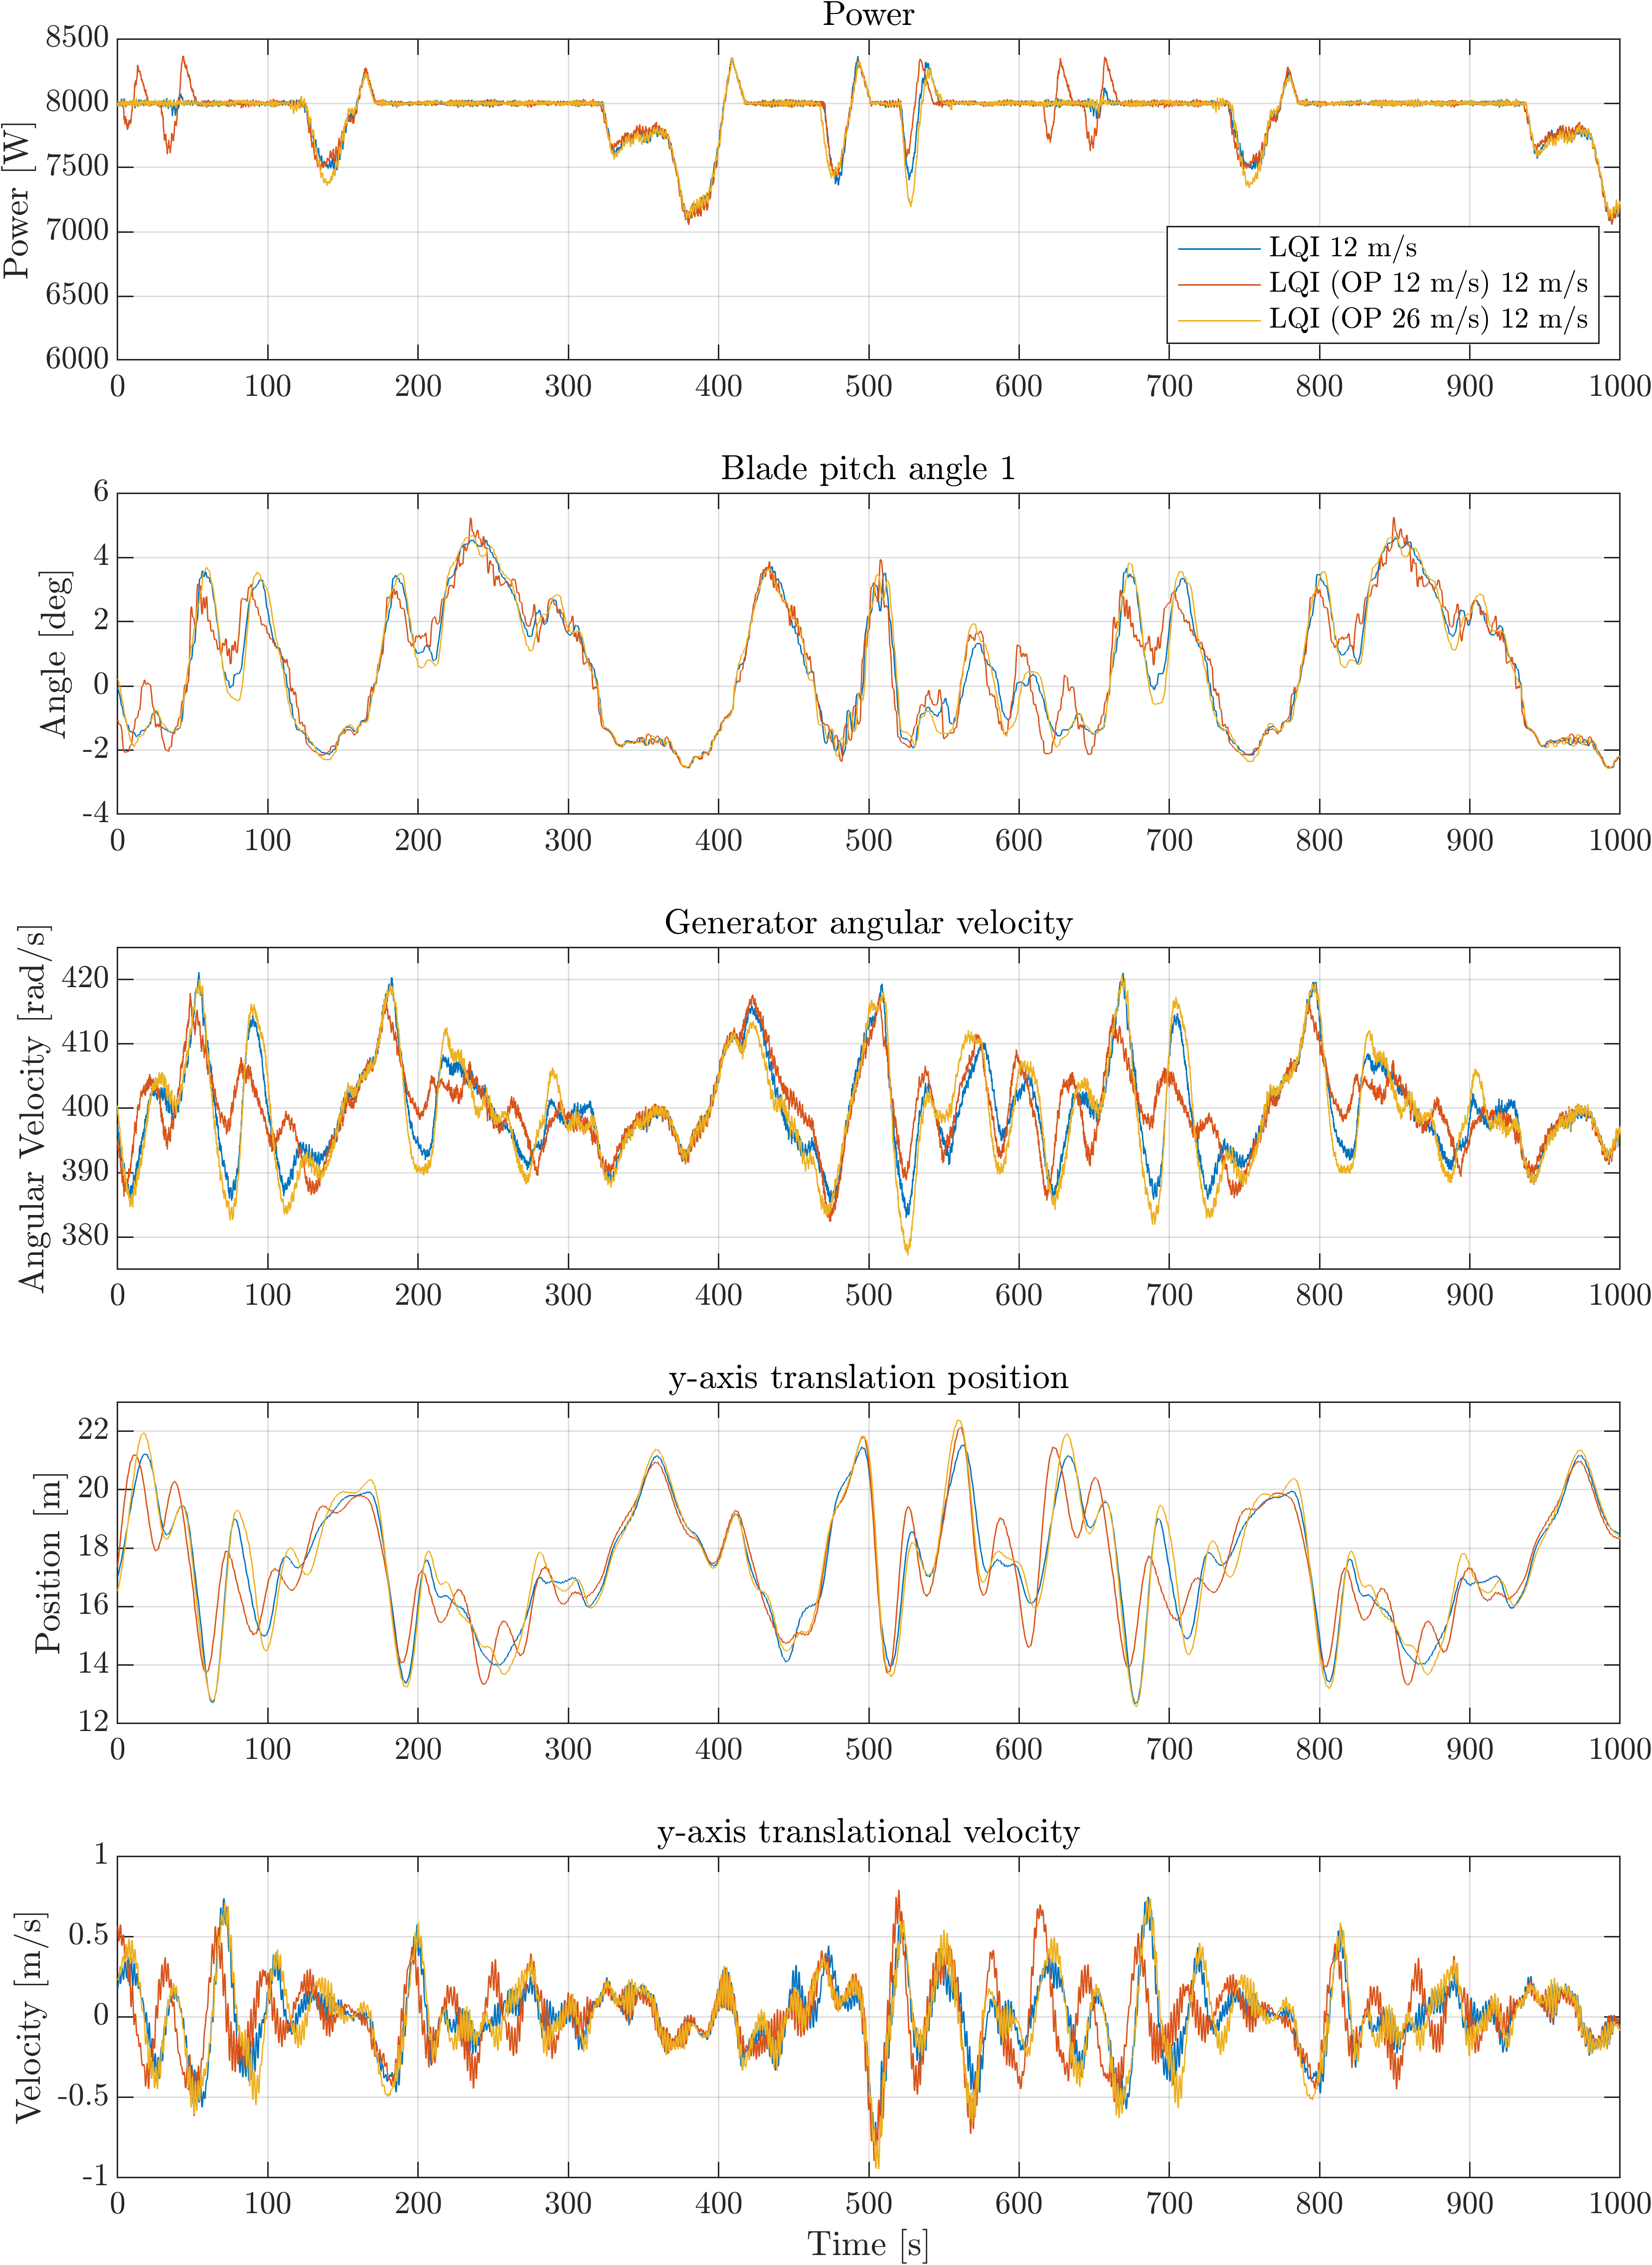
\includegraphics[width=0.7\linewidth]{Graphics/TestResults/VTSplotting/20_pow_th_w_py_vy.png}
	\caption{VTS simulation at 12 m/s mean wind speed for 1000 seconds. LQI parameters calculated for OPs at 16 m/s (blue), 12 m/s (red) and 26 m/s (yellow) are compared.}
	\label{fig:vts_20_pow_th_w_py_vy}
\end{figure}
\begin{figure}[ht]
	\centering
	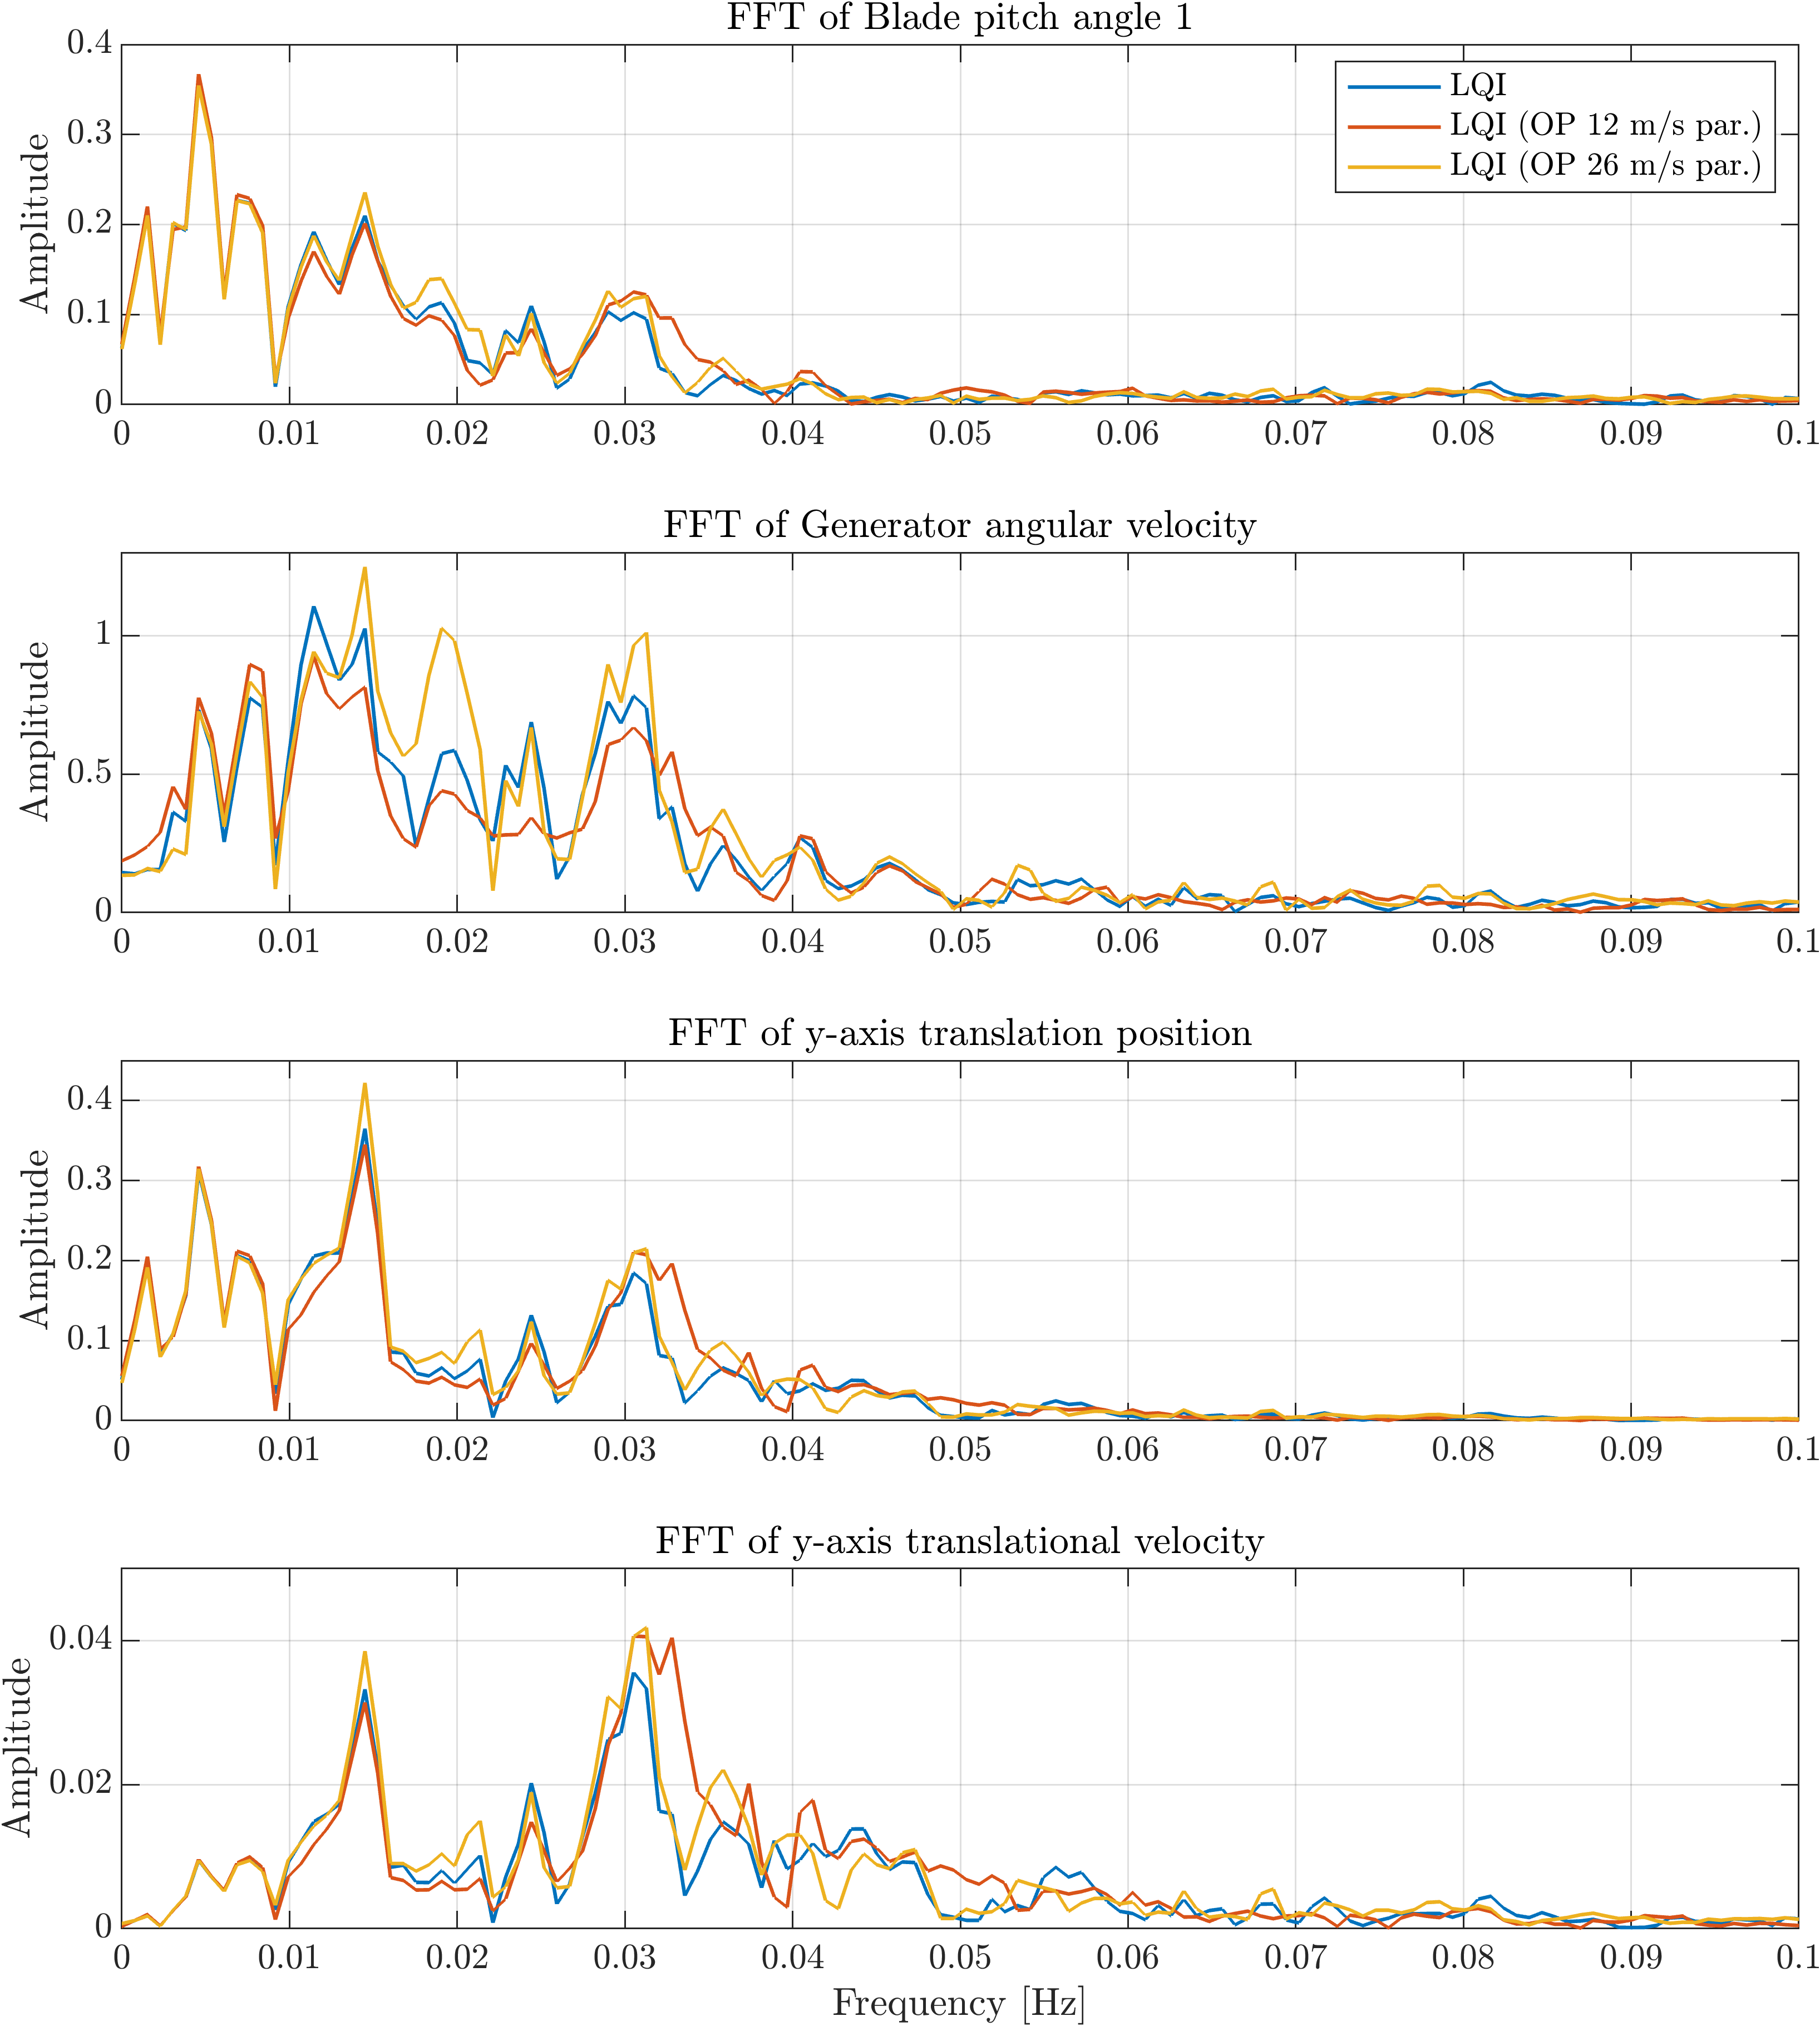
\includegraphics[width=0.7\linewidth]{Graphics/TestResults/VTSplotting/21_fft_th_w_py_vy.png}
	\caption{VTS simulation at 12 m/s mean wind speed with fourier transform zommed at the range 0 to 0.1 Hz. LQI parameters calculated for OPs at 16 m/s (blue), 12 m/s (red) and 26 m/s (yellow) are compared.}
	\label{fig:vts_21_fft_th_w_py_vy}
\end{figure}

\clearpage
In \cref{fig:vts_30_pow_th_w_py_vy} the 16 m/s and 26 m/s OP LQI parameter configurations are plotted at a mean wind speed of 26 m/s. The 12 m/s OP parameter configuration is left out since it had feedback weights so high that the system behaviour was oscillating out of control. At 26 m/s the turbine is de-rated as observed in the power output of the two remaining controllers which is constant around 6.8 MW. The generator speed set-point is also de-rated to around 370 rpm and relative high frequencies are present. The magnitude of fore-aft position oscillations is largely the same as at 16 m/s mean wind speed. In contrast to the expected much larger frequency content is present in the rotor speed and resultingly the blade pitch angle.

While not obvious it seems like the 26 m/s OP version has slightly lower generator speed error fluctuations. Interestingly when observing the fore-aft position and velocity the 26 m/s version seems to have smaller velocity oscillations but higher fluctuation in its position. When consulting the Fourier transform of the signal in \cref{fig:vts_31_fft_th_w_py_vy} it becomes apparent that the 26 m/s version does a better job with regards to dampening oscillations for both the 1st and 2nd mode. In both the generator speed and the fore-aft velocity the 3P frequency and second mode oscillations are greatly present. At 26 m/s mean wind speed the 3P frequency is even closer to the second mode due to the de-rated rotor speed. It is expected that the high second mode frequency content in the system is largely a result of the 3P excitation. When observing the rotor pitch it is confirmed that the 26 m/s controller version handles the fluctuations better by not transferring them as intensely to the blade pitch. The result is vastly smaller 2nd mode oscillations and smaller 3P oscillations. A phenomena which has not been observed in any of the other simulations is a large dominating 1P component in the pitch angle. The lack of frequency content at 1P in the generator speed and the fore-aft motion suggests that this results from another part of the Vestas controller. When observing \cref{fig:vts_10_th_w_py_vy} at 16 m/s the same kind of pitch activity is visible around 550 to 610 seconds.

\begin{figure}[ht]
	\centering
	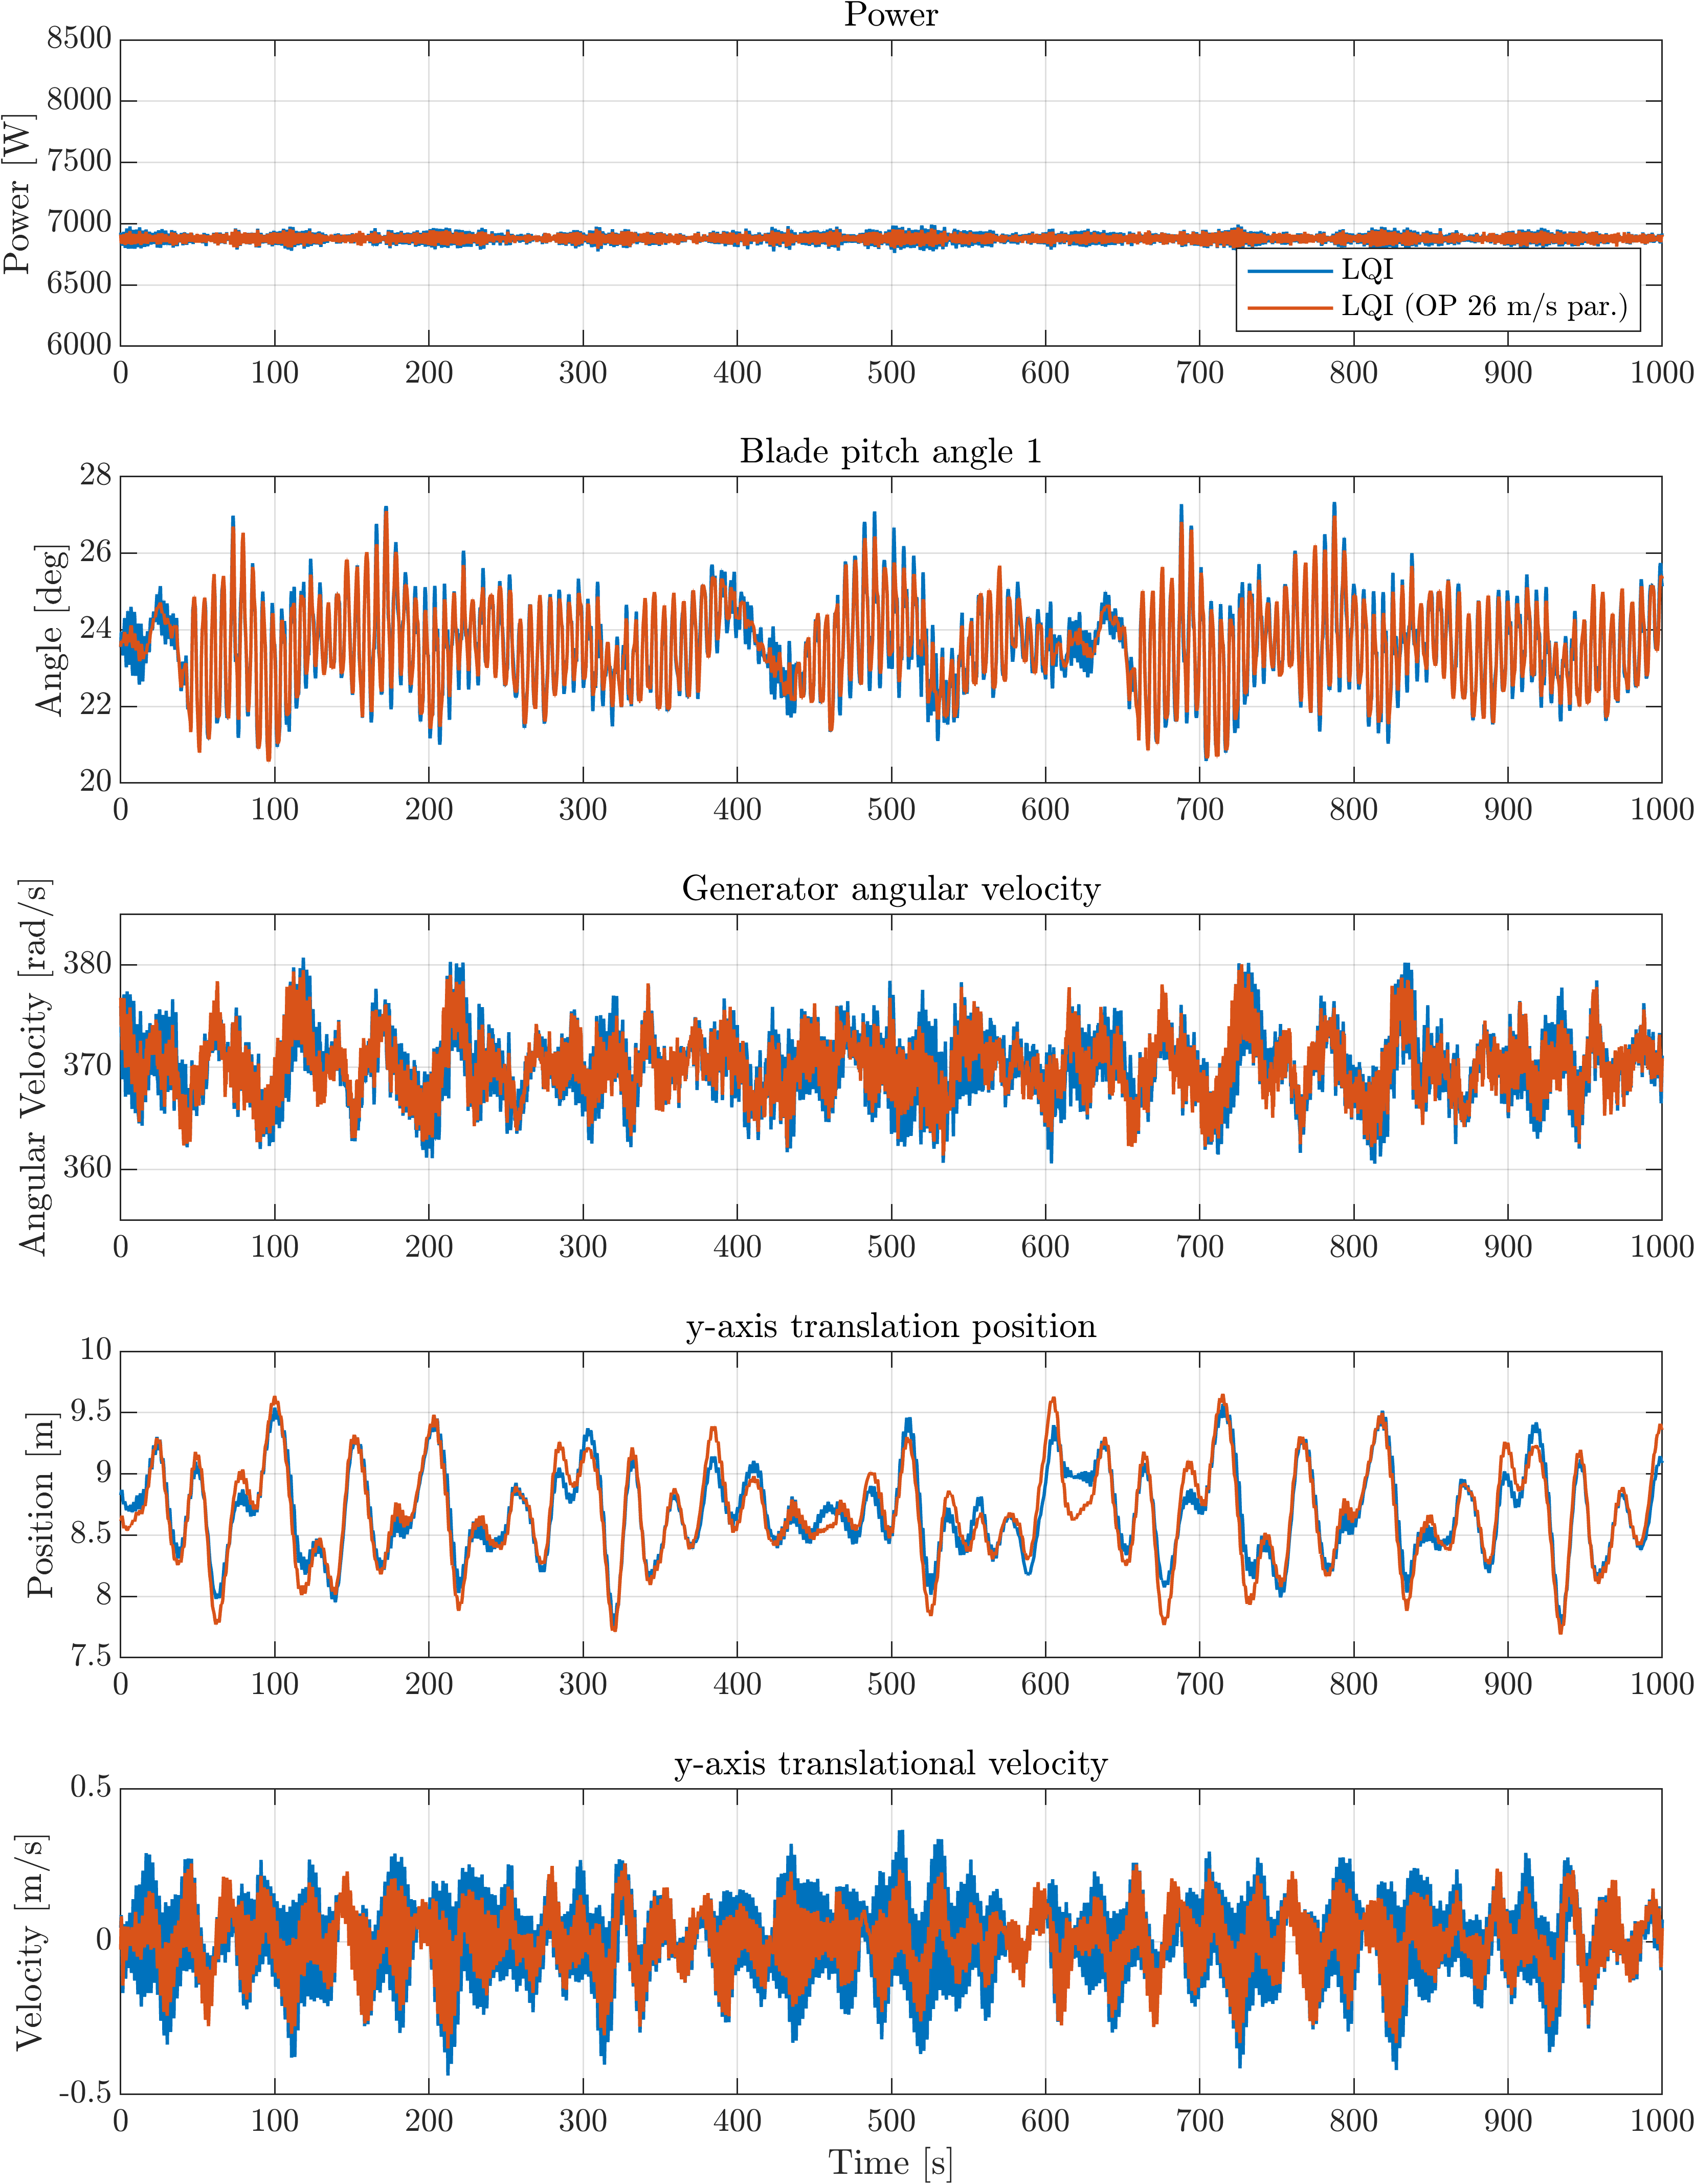
\includegraphics[width=0.7\linewidth]{Graphics/TestResults/VTSplotting/30_pow_th_w_py_vy.png}
	\caption{VTS simulation at 26 m/s mean wind speed. LQI parameters calculated for OPs at 16 m/s (blue), 12 m/s (red) and 26 m/s (yellow) are compared.}
	\label{fig:vts_30_pow_th_w_py_vy}
\end{figure}
\begin{figure}[ht]
	\centering
	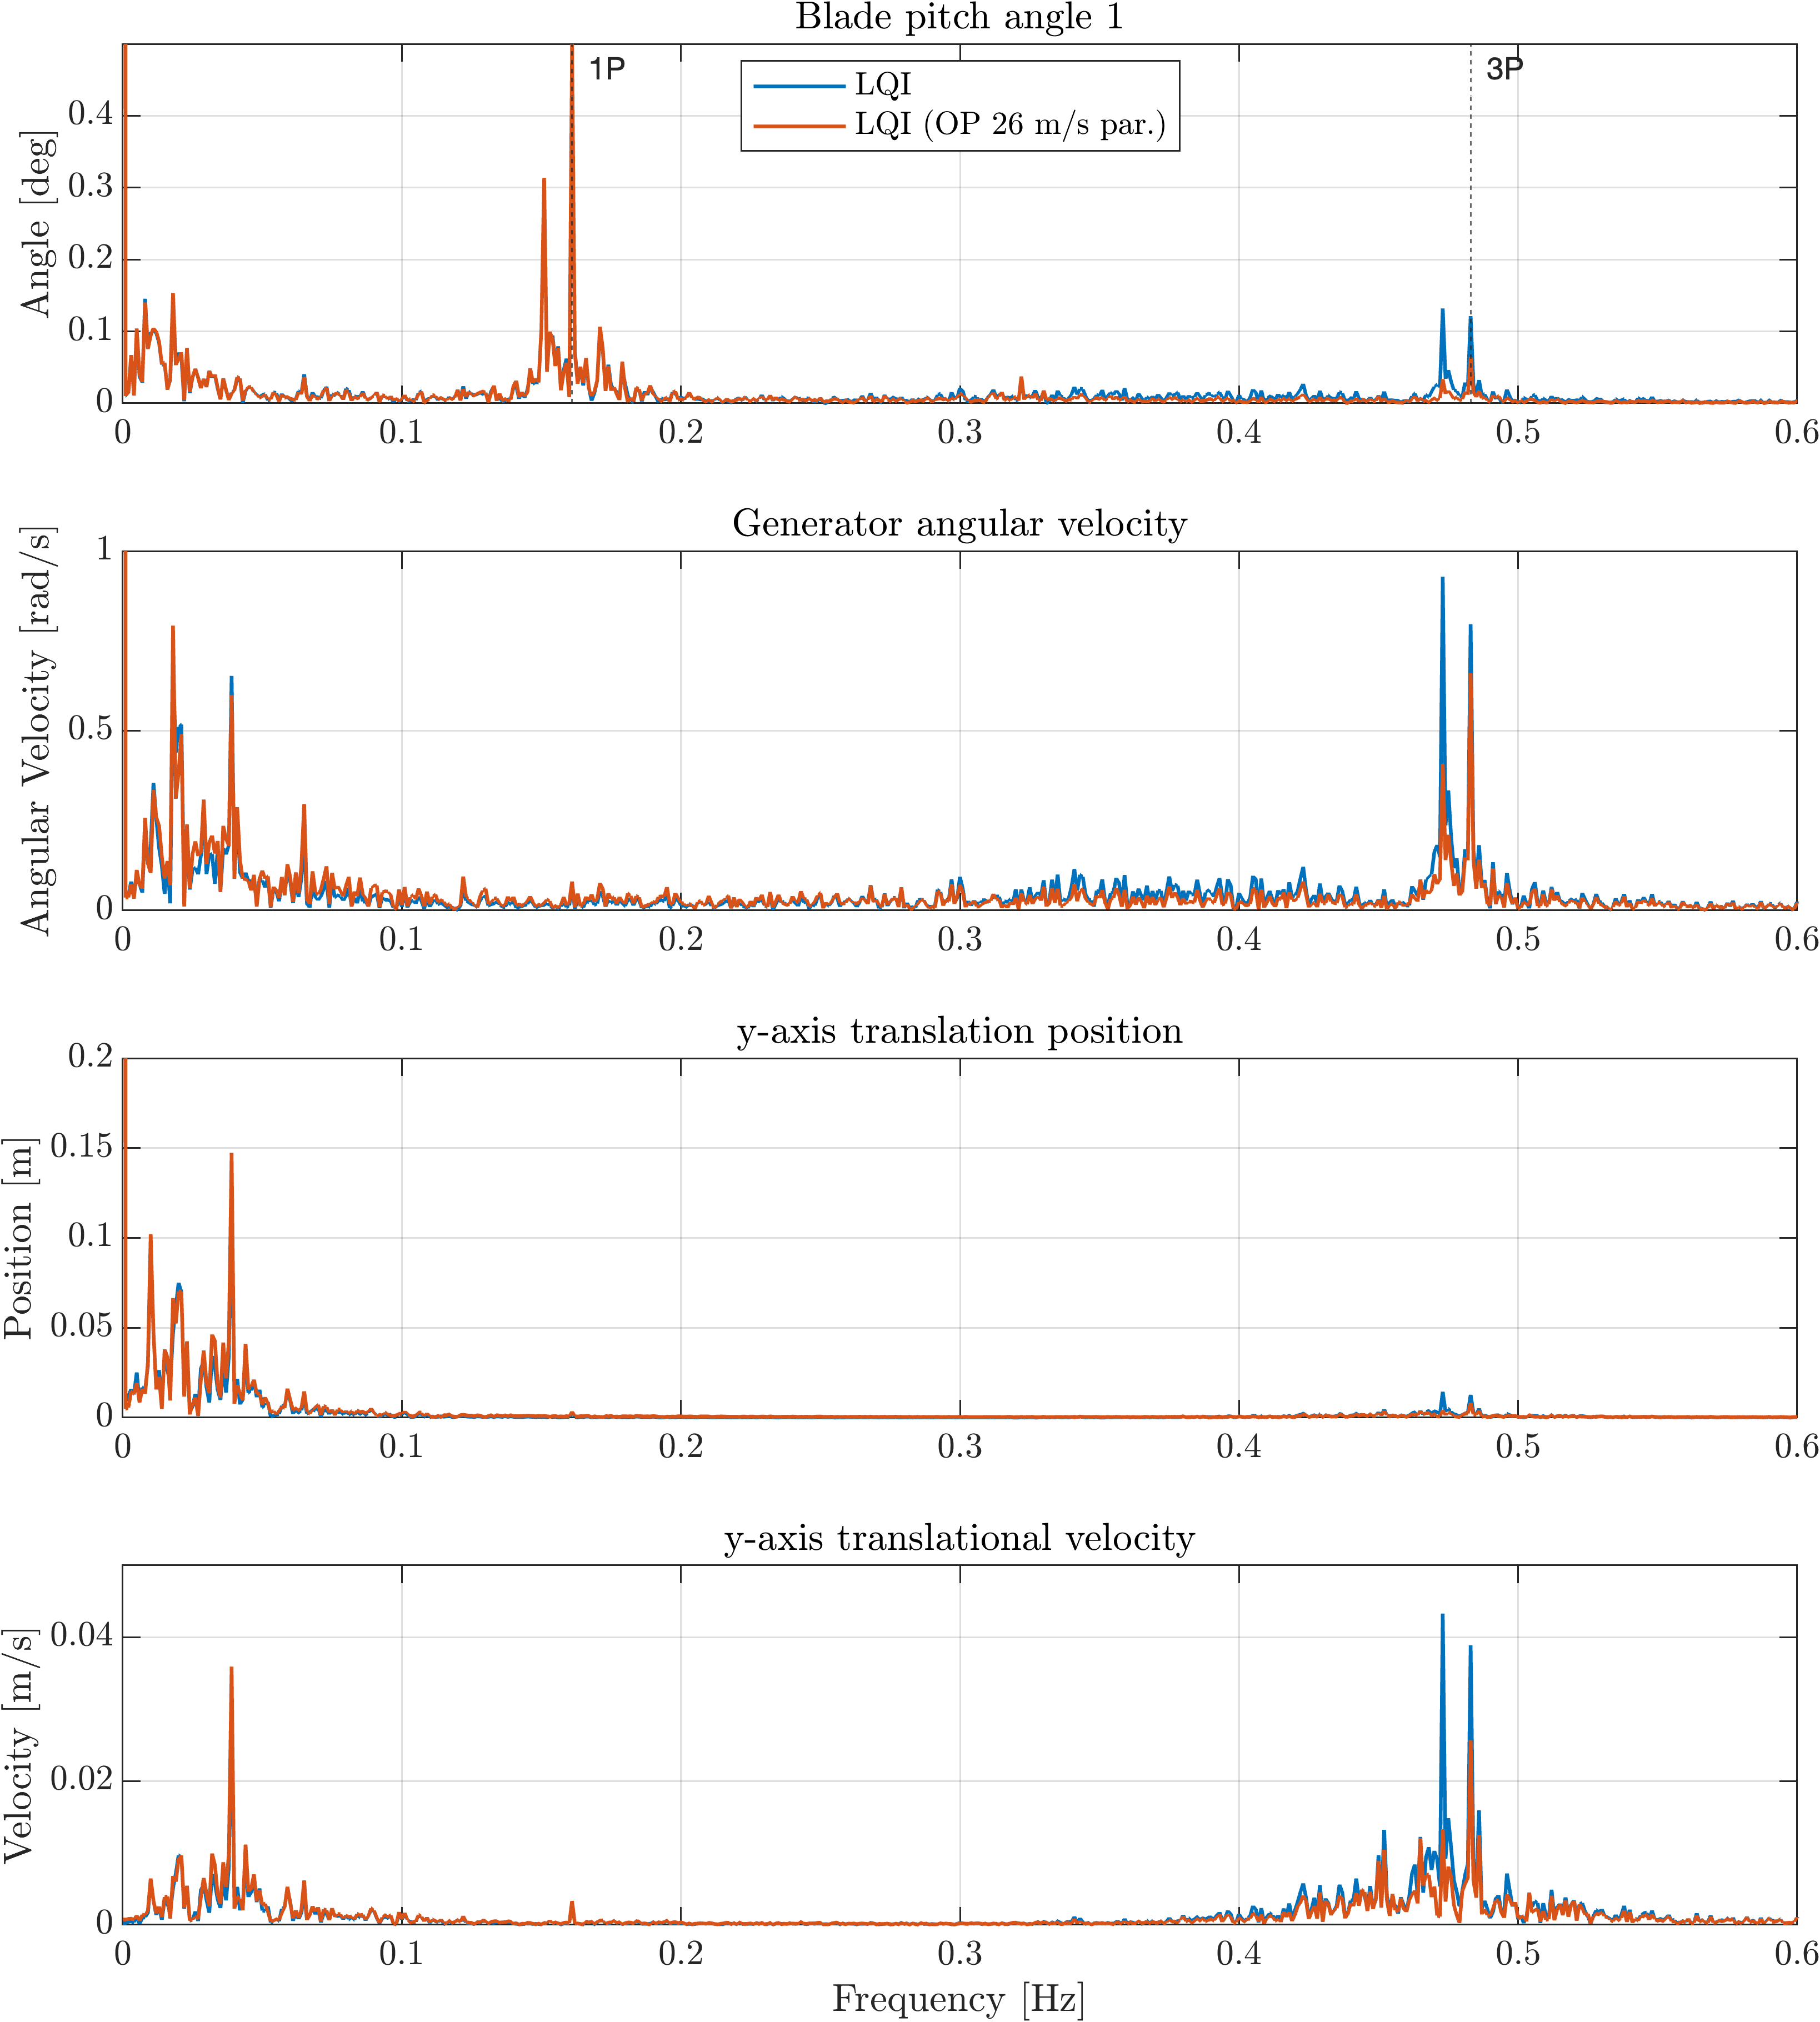
\includegraphics[width=0.7\linewidth]{Graphics/TestResults/VTSplotting/31_fft_th_w_py_vy.png}
	\caption{VTS simulation at 26 m/s mean wind speed. LQI parameters calculated for OPs at 16 m/s (blue), 12 m/s (red) and 26 m/s (yellow) are compared.}
	\label{fig:vts_31_fft_th_w_py_vy}
\end{figure}


\subsection{Test conclusion}


.. Greater performance is achieved at 12 m/s and 26 m/s mean wind speed if the LQI controller parameters are recalculated at the respective OPs which signifies that either gain scheduling or other methods should be employed to cover the whole turbine operating range. This comes to no surprise as the non-linear control authority of WT pitching is well known. It is assumed that greater performance can be achieved if LQI weight tuning was performed at the alternative wind speeds and perhaps if the fore-aft model fitting shown in \cref{sec:lin_fit_eval} was revisited as well.